\chapter{Diseño e implementación} % Main chapter title

\label{Chapter3} 

En este capítulo se describe el diseño e implementación de los dos modelos desarrollados en este trabajo. Debido a la naturaleza del trabajo, se divide el capítulo en dos secciones, una para la estimación de PLC y otra para la de CHF.

\section{Estimación de PLC}
En esta sección se describe el modelo para estimar PLC. Se presentan el pipeline de datos, la arquitectura de la DNN para estimar DNBR y fracción de vacío, su entrenamiento y optimización, y la implementación del modelo para el cálculo de PLC.

Se construyó un archivo Python llamado \texttt{plc.py} con funciones de ayuda, que permiten realizar el flujo completo en unas pocas líneas.

\subsection{Pipeline de datos}
Para la estimación de PLC, los datos provienen de simulaciones con COBRA3-CP de estados del reactor simulados para el diseño de la estrategia de recambio de combustibles. Se evaluaron 100 estados del reactor, cada uno implica 451 simulaciones.

De las simulaciones de COBRA3-CP, se extraen dos conjuntos de información: por un lado la información de entrada al código, y por otro la información de salida del código. La información de entrada al código de interés es: la zona hidráulica de ejecución, el perfil axial de potencia, el perfil por barra o radial de potencia, la potencia total del EECC, el caudal de entrada, la temperatura de entrada y la presión a la salida. En cuanto a la información de salida, se tiene: la fracción de vacío promedio a la salida del canal, y el MDNBR. Esta información es extraída para cada caso y canal.

Debido a que los datos de una estrategia están alrededor de los parámetros de operación del reactor, se agregó una varianza a los parámetros de potencia total, temperatura de entrada, y presión a la salida. Esto fue realizado por medio de un \textit{script} de Python, con las funciones \texttt{random()} y \texttt{randint()} de la biblioteca random, que proveen una distribución uniforme en el rango establecido. Se varió la potencia con aumentos de entre 5\% y 30\%, con intervalos de 5\%. La temperatura se varió en un intervalo uniforme entre 268 \degree C y 288 \degree C ($\pm$ 10 \degree C respecto de la temperatura nominal de operación), y la presión entre 105 bar y 125 bar ($\pm$ 10 bar respecto de la presión nominal de operación).

Las simulaciones se realizaron en paralelo y fueron procesadas al finalizar, para luego borrar el directorio de ejecución. De esta manera se evitó un excesivo volumen de datos en disco que no proveían valor.

La distribución de fracción de vacío y MDNBR obtenida se presenta en la figura \ref{fig:hist_void_mdnbr}. Se observa que el MDNBR tiene una fuerte dependencia con la ZH. Esto es esperable ya que cada ZH tiene una relación potencia-caudal característica, y los límites de DNBR son mayores cuanto más periférica la ZH. Es entonces un criterio de evaluación del modelo final la correcta predicción para cada ZH de la PLC. Por otro lado, la fracción de vacío presenta una distribución uniforme en casi todo el dominio, con un pico en 0, es decir líquido sin vapor a la salida del canal.

\begin{figure}[hbt]
    \centering
    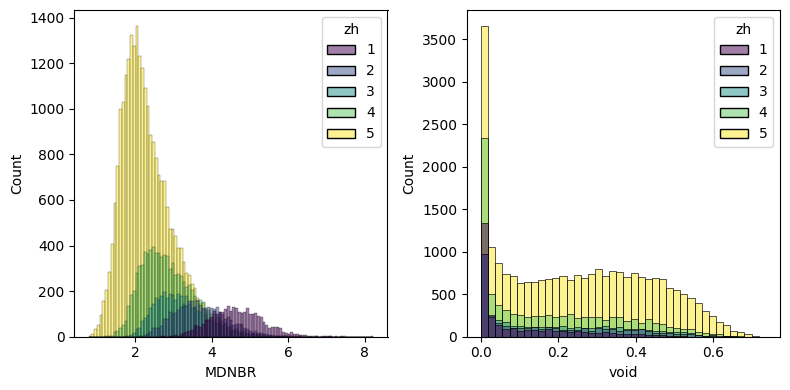
\includegraphics[width=\textwidth]{Figures/hist_void_mdnbr.png}
    \caption{Histogramas de fracción de vacío y MDNBR para las simulaciones con COBRA3-CP.}
    \label{fig:hist_void_mdnbr}
\end{figure}

Al realizar las simulaciones y procesarlas se generó un archivo con extensión \texttt{csv}, que tiene las siguientes columnas: \texttt{caso}, \texttt{canal}, \texttt{zh}, \texttt{pa1}, \texttt{...}, \texttt{pa22}, \texttt{pr1}, \texttt{...}, \texttt{pr37}, \texttt{power}, \texttt{void}, \texttt{caudal}, \texttt{temperatura}, \texttt{presion}, \texttt{MDNBR}. Este archivo fue importado como un objeto \texttt{pandas.DataFrame}, de la biblioteca pandas.

Se filtraron los resultados a utilizar por el valor de MDNBR y fracción de vacío, para utilizar sólo valores en el rango de interés al calcular las PLC. Los datos por fuera de estos rangos sirven de set adicional de evaluación, para determinar la capacidad de generalización del modelo por fuera del rango entrenado. Se filtraron los casos con MDNBR entre 1,7 y 2,5, o fracción de vacío entre 15\% y 35\%.

Con los resultados filtrados el pipeline es el siguiente:
\begin{enumerate}
    \item Conversión a tensores (\texttt{torch.tensor(, dtype=torch.float32)}) para las \textit{features} (todas las variables menos \texttt{MDNBR} y \texttt{void}) y \textit{target}.
    \item División entre \textit{train} y \textit{test} por medio de \texttt{train\_test\_split} de scikit-learn.
    \item Normalización de tensores de \textit{features} y \textit{targets} por medio de la función \texttt{plc.scale\_tensors()}, que utiliza por dentro \texttt{StandardScaler()} de scikit-learn.
\end{enumerate}

\subsection{Arquitectura del modelo, entrenamiento y optimización}
El estimador de PLC utiliza una arquitectura estándar de DNN, a partir del módulo \texttt{torch.nn.Sequential} y su método \texttt{add\_module()}. Los hiperparámetros a configurar son: cantidad de capas ocultas, cantidad de neuronas en las capas ocultas, función de activación, \textit{learning rate}, y tamaño del \textit{batch} de entrenamiento. 

En la figura \ref{fig:mlp-arquitectura} se esquematiza la arquitectura implementada. La entrada reúne las 63 variables mencionadas previamente: 22 componentes del perfil axial, las 37 componentes del perfil radial, y las condiciones de operación: potencia, caudal, temperatura y presión. A estas se aplica en la capa de entrada una función de activación $\sigma$. A continuación, estas variables ingresan en una red de \texttt{L} capas ocultas con \texttt{h} neuronas cada una, que aplican $\sigma$ en cada nodo. Por último la capa de salida tiene 2 variables: MDNBR y fracción de vacío.

% Arquitectura del perceptron multicapa (MLP).
%
% Fragmento para % Arquitectura del perceptron multicapa (MLP).
%
% Fragmento para % Arquitectura del perceptron multicapa (MLP).
%
% Fragmento para \input{Figures/mlp_arquitectura}.
% Requiere en el preambulo del documento principal:
%   \usepackage{tikz}
%   \usetikzlibrary{decorations.pathreplacing}
%   \usepackage{amsmath,amssymb}
%
% Entradas (63): pa_1..pa_22, pr_1..pr_37, power, caudal, temperatura, presion.
% Salidas (2):   MDNBR, void.
% h = hidden_dim, L = cantidad de bloques lineal+activacion repetidos,
% sigma = funcion de activacion.
% La red tiene L+1 capas ocultas: la primera proviene de la capa lineal de
% entrada y las L restantes del bloque repetido.

\begin{figure}[htbp]
  \centering
  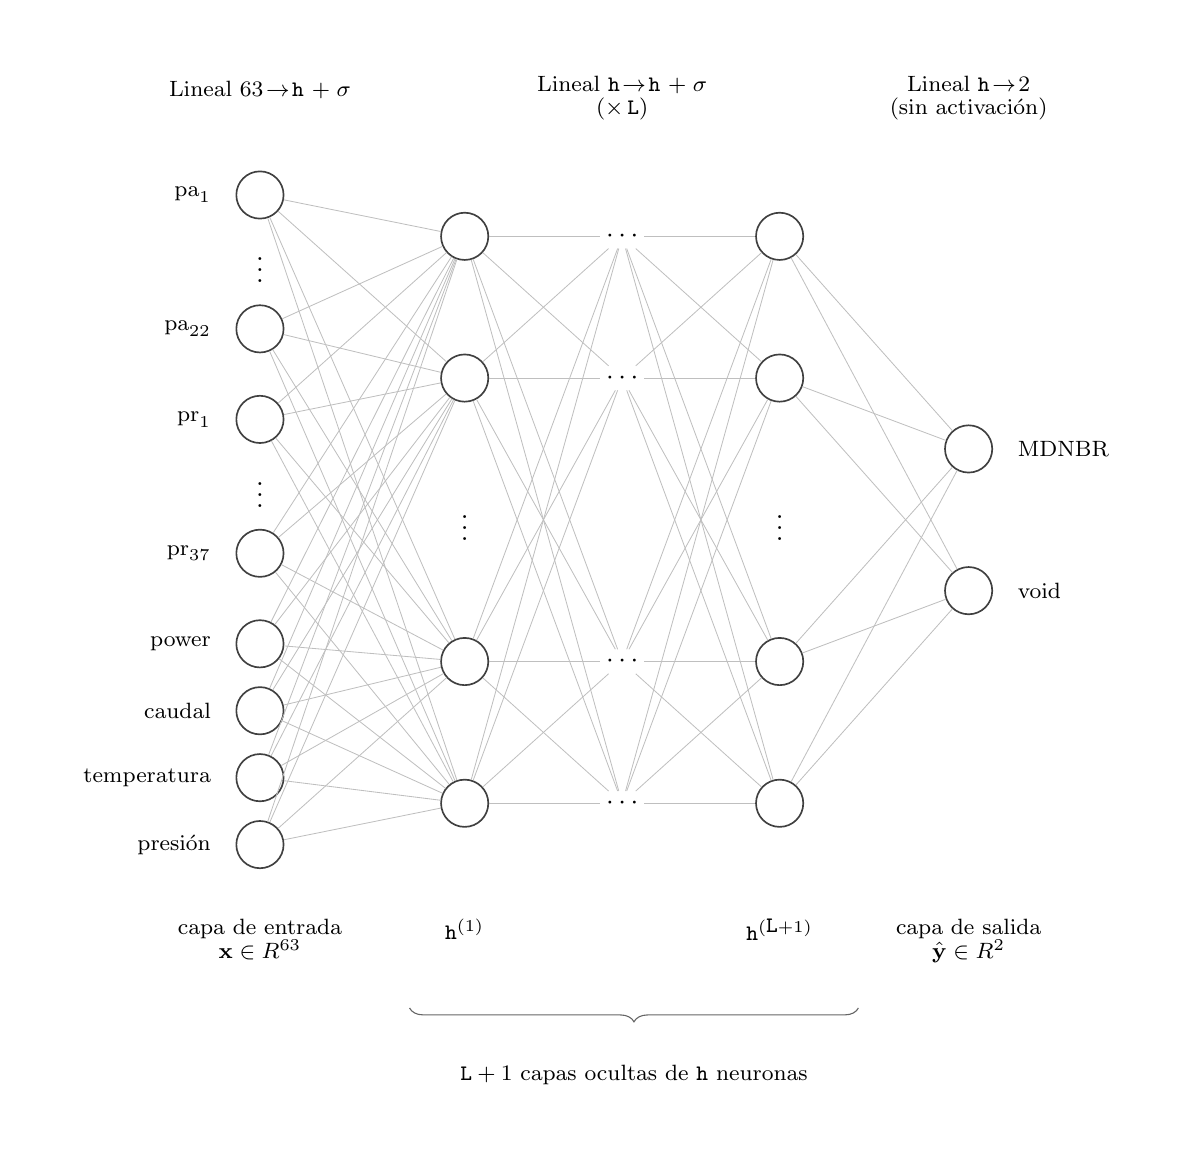
\begin{tikzpicture}[
      neurona/.style  = {circle, draw=black!75, fill=white, line width=0.6pt,
                         minimum size=6mm, inner sep=0pt},
      conexion/.style = {draw=black!25, line width=0.3pt},
      puntos/.style   = {inner sep=2pt},
      nombre/.style   = {font=\footnotesize},
      texto/.style    = {font=\footnotesize, align=center},
    ]
    \useasboundingbox (-2.95,-7.7) rectangle (11.6,6.25);

    %------------------------------------------------ capa de entrada (63)
    \foreach \y/\etq [count=\i] in {%
        4.125/$\mathrm{pa}_{1}$,
        2.425/$\mathrm{pa}_{22}$,
        1.275/$\mathrm{pr}_{1}$,
        -0.425/$\mathrm{pr}_{37}$,
        -1.575/power,
        -2.425/caudal,
        -3.275/temperatura,
        -4.125/presi\'on} {
      \node[neurona] (I-\i) at (0,\y) {};
      \node[nombre, anchor=east] at (-0.5,\y) {\etq};
    }
    \node[puntos] at (0,3.275) {$\vdots$};
    \node[puntos] at (0,0.425) {$\vdots$};

    %------------------------------------------------ primera capa oculta
    \foreach \y [count=\i] in {3.6, 1.8, -1.8, -3.6}
      \node[neurona] (H-\i) at (2.6,\y) {};
    \node[puntos] at (2.6,0) {$\vdots$};

    %------------------------------------------------ capas ocultas elididas
    \foreach \y [count=\i] in {3.6, 1.8, -1.8, -3.6}
      \node[puntos] (D-\i) at (4.6,\y) {$\cdots$};

    %------------------------------------------------ ultima capa oculta
    \foreach \y [count=\i] in {3.6, 1.8, -1.8, -3.6}
      \node[neurona] (G-\i) at (6.6,\y) {};
    \node[puntos] at (6.6,0) {$\vdots$};

    %------------------------------------------------ capa de salida (2)
    \foreach \y/\etq [count=\i] in {0.9/MDNBR, -0.9/void} {
      \node[neurona] (O-\i) at (9.0,\y) {};
      \node[nombre, anchor=west] at (9.5,\y) {\etq};
    }

    %------------------------------------------------ conexiones densas
    \foreach \a in {1,...,8}
      \foreach \b in {1,...,4}
        \draw[conexion] (I-\a) -- (H-\b);
    \foreach \a in {1,...,4}
      \foreach \b in {1,...,4} {
        \draw[conexion] (H-\a) -- (D-\b);
        \draw[conexion] (D-\a) -- (G-\b);
      }
    \foreach \a in {1,...,4}
      \foreach \b in {1,2}
        \draw[conexion] (G-\a) -- (O-\b);

    %------------------------------------------------ transformaciones
    \node[texto, anchor=south] at (0,4.95)
      {Lineal $63\!\to\!\texttt{h}$ $+\;\sigma$\\[-1pt]};
    \node[texto, anchor=south] at (4.6,4.95)
      {Lineal $\texttt{h}\!\to\!\texttt{h}$ $+\;\sigma$\\[-1pt] ($\times\,\texttt{L}$)};
    \node[texto, anchor=south] at (9,4.95)
      {Lineal $\texttt{h}\!\to\!2$\\[-1pt] (sin activaci\'on)};

    %------------------------------------------------ nombres de las capas
    \node[texto, anchor=north] at (0,-4.95)
      {capa de entrada\\[-1pt] $\mathbf{x}\in\mathbb{R}^{63}$};
    \node[texto, anchor=north] at (2.6,-4.95) {$\mathbf{\texttt{h}}^{(1)}$};
    \node[texto, anchor=north] at (6.6,-4.95) {$\mathbf{\texttt{h}}^{(\texttt{L}+1)}$};
    \node[texto, anchor=north] at (9.0,-4.95)
      {capa de salida\\[-1pt] $\hat{\mathbf{y}}\in\mathbb{R}^{2}$};

    %------------------------------------------------ llave de capas ocultas
    \draw[decorate, decoration={brace, amplitude=5pt, mirror}, draw=black!60]
      (1.9,-6.2) -- (7.6,-6.2);
    \node[texto, anchor=north] at (4.75,-6.8)
      {$\texttt{L}+1$ capas ocultas de \texttt{h} neuronas};
  \end{tikzpicture}
  \caption{Arquitectura de la DNN para estimación de MDNBR y fracción de vacío, para predicción de PLC.}
  \label{fig:mlp-arquitectura}
\end{figure}
.
% Requiere en el preambulo del documento principal:
%   \usepackage{tikz}
%   \usetikzlibrary{decorations.pathreplacing}
%   \usepackage{amsmath,amssymb}
%
% Entradas (63): pa_1..pa_22, pr_1..pr_37, power, caudal, temperatura, presion.
% Salidas (2):   MDNBR, void.
% h = hidden_dim, L = cantidad de bloques lineal+activacion repetidos,
% sigma = funcion de activacion.
% La red tiene L+1 capas ocultas: la primera proviene de la capa lineal de
% entrada y las L restantes del bloque repetido.

\begin{figure}[htbp]
  \centering
  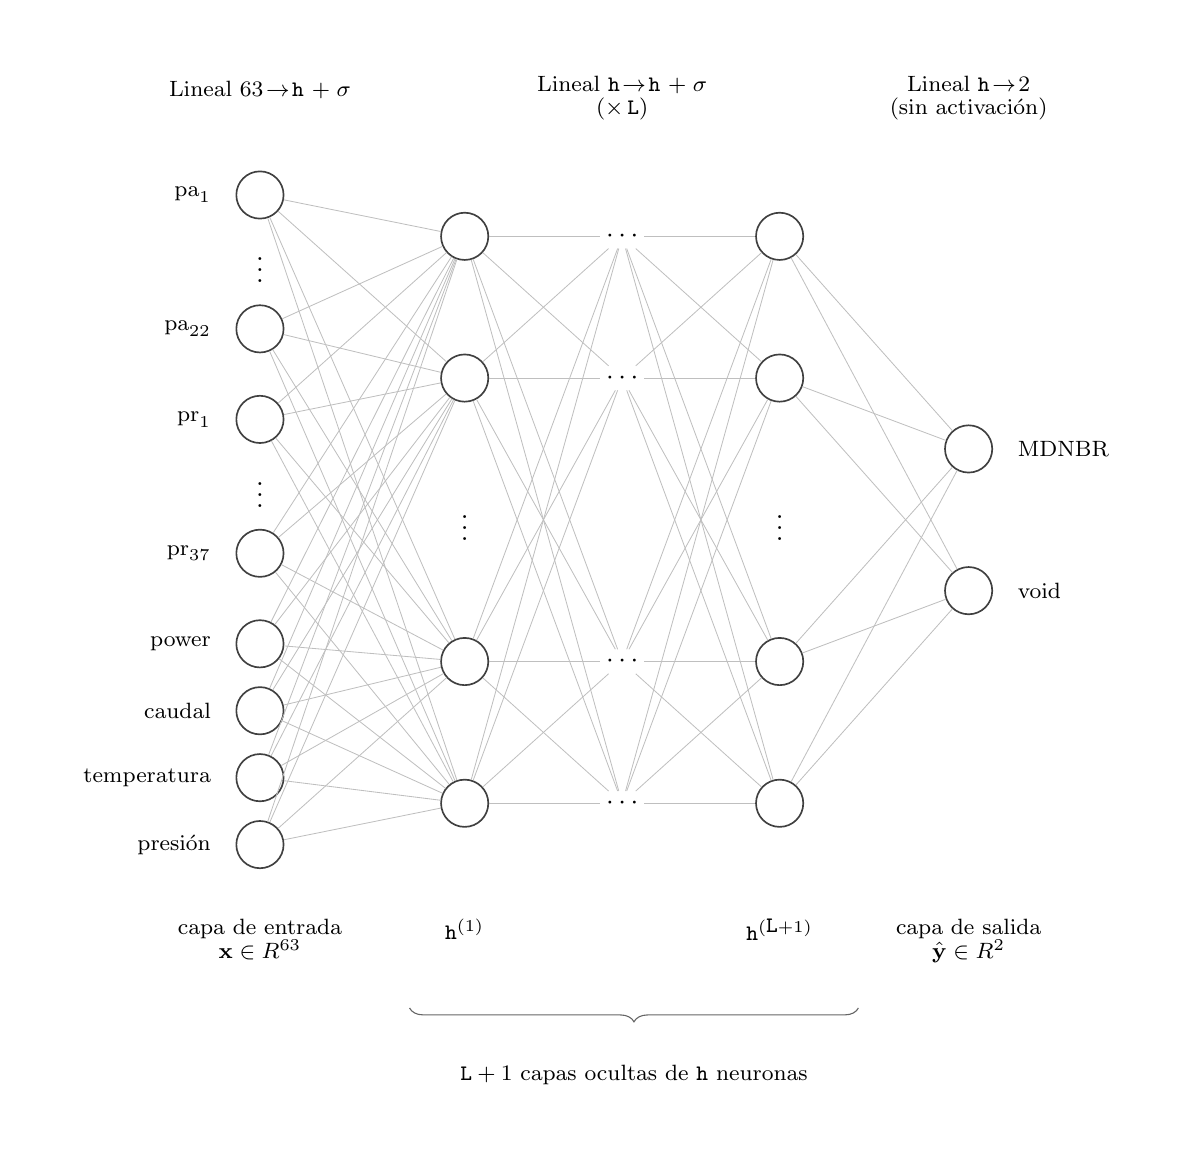
\begin{tikzpicture}[
      neurona/.style  = {circle, draw=black!75, fill=white, line width=0.6pt,
                         minimum size=6mm, inner sep=0pt},
      conexion/.style = {draw=black!25, line width=0.3pt},
      puntos/.style   = {inner sep=2pt},
      nombre/.style   = {font=\footnotesize},
      texto/.style    = {font=\footnotesize, align=center},
    ]
    \useasboundingbox (-2.95,-7.7) rectangle (11.6,6.25);

    %------------------------------------------------ capa de entrada (63)
    \foreach \y/\etq [count=\i] in {%
        4.125/$\mathrm{pa}_{1}$,
        2.425/$\mathrm{pa}_{22}$,
        1.275/$\mathrm{pr}_{1}$,
        -0.425/$\mathrm{pr}_{37}$,
        -1.575/power,
        -2.425/caudal,
        -3.275/temperatura,
        -4.125/presi\'on} {
      \node[neurona] (I-\i) at (0,\y) {};
      \node[nombre, anchor=east] at (-0.5,\y) {\etq};
    }
    \node[puntos] at (0,3.275) {$\vdots$};
    \node[puntos] at (0,0.425) {$\vdots$};

    %------------------------------------------------ primera capa oculta
    \foreach \y [count=\i] in {3.6, 1.8, -1.8, -3.6}
      \node[neurona] (H-\i) at (2.6,\y) {};
    \node[puntos] at (2.6,0) {$\vdots$};

    %------------------------------------------------ capas ocultas elididas
    \foreach \y [count=\i] in {3.6, 1.8, -1.8, -3.6}
      \node[puntos] (D-\i) at (4.6,\y) {$\cdots$};

    %------------------------------------------------ ultima capa oculta
    \foreach \y [count=\i] in {3.6, 1.8, -1.8, -3.6}
      \node[neurona] (G-\i) at (6.6,\y) {};
    \node[puntos] at (6.6,0) {$\vdots$};

    %------------------------------------------------ capa de salida (2)
    \foreach \y/\etq [count=\i] in {0.9/MDNBR, -0.9/void} {
      \node[neurona] (O-\i) at (9.0,\y) {};
      \node[nombre, anchor=west] at (9.5,\y) {\etq};
    }

    %------------------------------------------------ conexiones densas
    \foreach \a in {1,...,8}
      \foreach \b in {1,...,4}
        \draw[conexion] (I-\a) -- (H-\b);
    \foreach \a in {1,...,4}
      \foreach \b in {1,...,4} {
        \draw[conexion] (H-\a) -- (D-\b);
        \draw[conexion] (D-\a) -- (G-\b);
      }
    \foreach \a in {1,...,4}
      \foreach \b in {1,2}
        \draw[conexion] (G-\a) -- (O-\b);

    %------------------------------------------------ transformaciones
    \node[texto, anchor=south] at (0,4.95)
      {Lineal $63\!\to\!\texttt{h}$ $+\;\sigma$\\[-1pt]};
    \node[texto, anchor=south] at (4.6,4.95)
      {Lineal $\texttt{h}\!\to\!\texttt{h}$ $+\;\sigma$\\[-1pt] ($\times\,\texttt{L}$)};
    \node[texto, anchor=south] at (9,4.95)
      {Lineal $\texttt{h}\!\to\!2$\\[-1pt] (sin activaci\'on)};

    %------------------------------------------------ nombres de las capas
    \node[texto, anchor=north] at (0,-4.95)
      {capa de entrada\\[-1pt] $\mathbf{x}\in\mathbb{R}^{63}$};
    \node[texto, anchor=north] at (2.6,-4.95) {$\mathbf{\texttt{h}}^{(1)}$};
    \node[texto, anchor=north] at (6.6,-4.95) {$\mathbf{\texttt{h}}^{(\texttt{L}+1)}$};
    \node[texto, anchor=north] at (9.0,-4.95)
      {capa de salida\\[-1pt] $\hat{\mathbf{y}}\in\mathbb{R}^{2}$};

    %------------------------------------------------ llave de capas ocultas
    \draw[decorate, decoration={brace, amplitude=5pt, mirror}, draw=black!60]
      (1.9,-6.2) -- (7.6,-6.2);
    \node[texto, anchor=north] at (4.75,-6.8)
      {$\texttt{L}+1$ capas ocultas de \texttt{h} neuronas};
  \end{tikzpicture}
  \caption{Arquitectura de la DNN para estimación de MDNBR y fracción de vacío, para predicción de PLC.}
  \label{fig:mlp-arquitectura}
\end{figure}
.
% Requiere en el preambulo del documento principal:
%   \usepackage{tikz}
%   \usetikzlibrary{decorations.pathreplacing}
%   \usepackage{amsmath,amssymb}
%
% Entradas (63): pa_1..pa_22, pr_1..pr_37, power, caudal, temperatura, presion.
% Salidas (2):   MDNBR, void.
% h = hidden_dim, L = cantidad de bloques lineal+activacion repetidos,
% sigma = funcion de activacion.
% La red tiene L+1 capas ocultas: la primera proviene de la capa lineal de
% entrada y las L restantes del bloque repetido.

\begin{figure}[htbp]
  \centering
  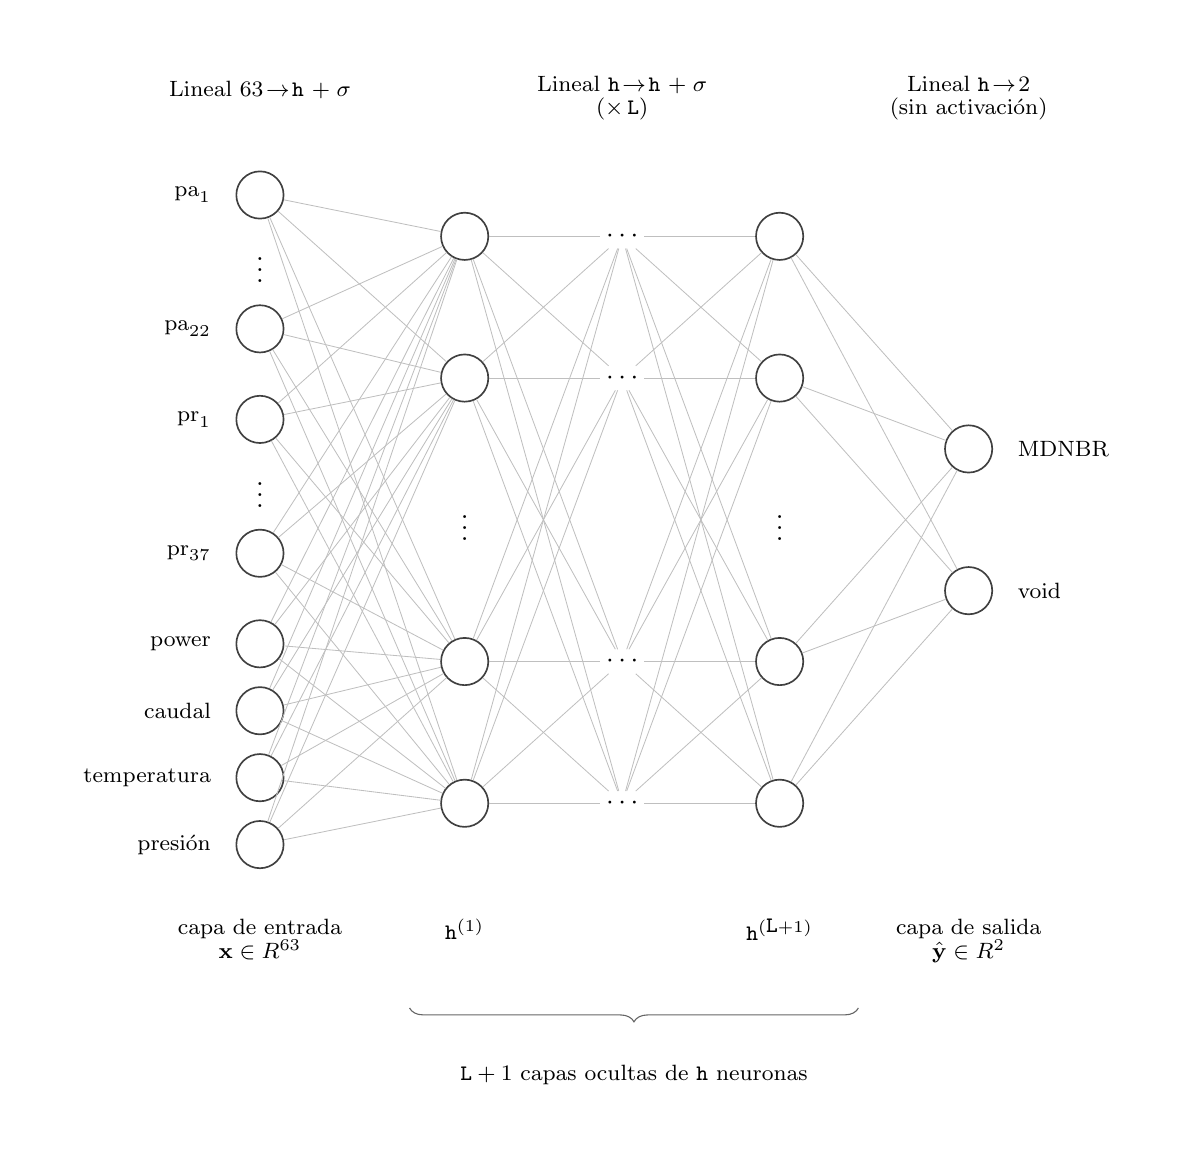
\begin{tikzpicture}[
      neurona/.style  = {circle, draw=black!75, fill=white, line width=0.6pt,
                         minimum size=6mm, inner sep=0pt},
      conexion/.style = {draw=black!25, line width=0.3pt},
      puntos/.style   = {inner sep=2pt},
      nombre/.style   = {font=\footnotesize},
      texto/.style    = {font=\footnotesize, align=center},
    ]
    \useasboundingbox (-2.95,-7.7) rectangle (11.6,6.25);

    %------------------------------------------------ capa de entrada (63)
    \foreach \y/\etq [count=\i] in {%
        4.125/$\mathrm{pa}_{1}$,
        2.425/$\mathrm{pa}_{22}$,
        1.275/$\mathrm{pr}_{1}$,
        -0.425/$\mathrm{pr}_{37}$,
        -1.575/power,
        -2.425/caudal,
        -3.275/temperatura,
        -4.125/presi\'on} {
      \node[neurona] (I-\i) at (0,\y) {};
      \node[nombre, anchor=east] at (-0.5,\y) {\etq};
    }
    \node[puntos] at (0,3.275) {$\vdots$};
    \node[puntos] at (0,0.425) {$\vdots$};

    %------------------------------------------------ primera capa oculta
    \foreach \y [count=\i] in {3.6, 1.8, -1.8, -3.6}
      \node[neurona] (H-\i) at (2.6,\y) {};
    \node[puntos] at (2.6,0) {$\vdots$};

    %------------------------------------------------ capas ocultas elididas
    \foreach \y [count=\i] in {3.6, 1.8, -1.8, -3.6}
      \node[puntos] (D-\i) at (4.6,\y) {$\cdots$};

    %------------------------------------------------ ultima capa oculta
    \foreach \y [count=\i] in {3.6, 1.8, -1.8, -3.6}
      \node[neurona] (G-\i) at (6.6,\y) {};
    \node[puntos] at (6.6,0) {$\vdots$};

    %------------------------------------------------ capa de salida (2)
    \foreach \y/\etq [count=\i] in {0.9/MDNBR, -0.9/void} {
      \node[neurona] (O-\i) at (9.0,\y) {};
      \node[nombre, anchor=west] at (9.5,\y) {\etq};
    }

    %------------------------------------------------ conexiones densas
    \foreach \a in {1,...,8}
      \foreach \b in {1,...,4}
        \draw[conexion] (I-\a) -- (H-\b);
    \foreach \a in {1,...,4}
      \foreach \b in {1,...,4} {
        \draw[conexion] (H-\a) -- (D-\b);
        \draw[conexion] (D-\a) -- (G-\b);
      }
    \foreach \a in {1,...,4}
      \foreach \b in {1,2}
        \draw[conexion] (G-\a) -- (O-\b);

    %------------------------------------------------ transformaciones
    \node[texto, anchor=south] at (0,4.95)
      {Lineal $63\!\to\!\texttt{h}$ $+\;\sigma$\\[-1pt]};
    \node[texto, anchor=south] at (4.6,4.95)
      {Lineal $\texttt{h}\!\to\!\texttt{h}$ $+\;\sigma$\\[-1pt] ($\times\,\texttt{L}$)};
    \node[texto, anchor=south] at (9,4.95)
      {Lineal $\texttt{h}\!\to\!2$\\[-1pt] (sin activaci\'on)};

    %------------------------------------------------ nombres de las capas
    \node[texto, anchor=north] at (0,-4.95)
      {capa de entrada\\[-1pt] $\mathbf{x}\in\mathbb{R}^{63}$};
    \node[texto, anchor=north] at (2.6,-4.95) {$\mathbf{\texttt{h}}^{(1)}$};
    \node[texto, anchor=north] at (6.6,-4.95) {$\mathbf{\texttt{h}}^{(\texttt{L}+1)}$};
    \node[texto, anchor=north] at (9.0,-4.95)
      {capa de salida\\[-1pt] $\hat{\mathbf{y}}\in\mathbb{R}^{2}$};

    %------------------------------------------------ llave de capas ocultas
    \draw[decorate, decoration={brace, amplitude=5pt, mirror}, draw=black!60]
      (1.9,-6.2) -- (7.6,-6.2);
    \node[texto, anchor=north] at (4.75,-6.8)
      {$\texttt{L}+1$ capas ocultas de \texttt{h} neuronas};
  \end{tikzpicture}
  \caption{Arquitectura de la DNN para estimación de MDNBR y fracción de vacío, para predicción de PLC.}
  \label{fig:mlp-arquitectura}
\end{figure}


Para el armado de la arquitectura se desarrolló la función \texttt{plc.build\_model} que permite en una línea obtener el modelo con los hiperparámetros deseados.

Para entrenar al modelo se utilizó Adam \citep{kingma2015adam} como optimizador, debido a su alta capacidad y adopción en casos clásicos de DNN. Como función de pérdida se utilizó la raíz del error cuadrático medio (RMSE, del inglés \textit{Root Mean Squared Error}), debido a que penaliza fuertemente los errores grandes y tiene magnitud del orden de las variables a optimizar.

Durante el entrenamiento se evalúa, además de la función de pérdida, el coeficiente de correlación $\text{R}^2$, tanto para el set de entrenamiento como el de evaluación. Al predecir sobre el set de evaluación, se utiliza la condición \texttt{torch.no\_grad()} para evitar que se aprenda de este set de datos y genere \textit{data leakage}. Se desarrolló la función de ayuda \texttt{plc.train\_model} para realizar el entrenamiento sobre la cantidad de épocas deseadas de forma sencilla.

La definición de los hiperparámetros se realiza por medio de su optimización con optuna. Para ello se plantea un estudio de hiperparámetros con 50 \textit{trials} de 200 épocas cada uno. Se consideraron DNN con entre 2 y 15 capas ocultas, de entre 32 y 512 neuronas cada uno, con un \textit{learning rate} de entre $10^{-2}$ y $10^{-5}$ y \textit{batches} de entrenamiento de entre 16 y 236.
Las funciones de activación consideradas fueron: ReLU \citep{nair2010rectified}, GELU \citep{hendrycks2016gaussian}, SiLU/Swish \citep{elfwing2018sigmoid}, Tanh, Leaky ReLU \citep{maas2013rectifier} y ELU \citep{clevert2015fast}.

En el capítulo \ref{Chapter4} se presentan los resultados de la optimización realizada.

\subsection{Integración e implementación del sistema}
La integración consiste en realizar el lazo de cálculo de PLC de COBRA, pero con la DNN entrenada en su lugar. Se tiene un lazo para cada límite de PLC, pero son idénticos en concepto. Únicamente se debe modificar la variable objetivo según si es criterio de DNB o de fracción de vacío.

El lazo de cálculo se esquematiza en la figura \ref{fig:dnb-dnn-loop}. En la misma se observa que en primer lugar se deben definir las condiciones operativas, esto es, temperatura y presión, y el límite objetivo, ya sea de MDNBR o de fracción de vacío. Luego se realizan dos cálculos, uno de piso y otro de techo, donde se evalúan los flujos de calor mínimo y máximo. Estos valores se establecen de antemano y se deben proveer valores que contengan al flujo de calor correspondiente al límite objetivo, por lo que un rango amplio es recomendable. Se obtiene el valor del límite para el flujo de calor mínimo y máximo, y por el método de la secante se estima el flujo de calor que debería obtener el límite objetivo. Se recalcula el caudal másico con dicho flujo de calor, y se vuelve a estimar el límite. Si se obtiene convergencia tanto en el límite objetivo, como en caudal y flujo de calor, se termina el lazo de cálculo. Si no se obtiene convergencia, se realiza una nueva iteración del método de la secante.

Para calcular el flujo másico en función del flujo de calor, se recurre a la relación caudal-potencia desarrollada por INVAP en \citep{invap_caudal_potencia}, donde para cada ZH y condición operativa se tiene una tabla para interpolar caudal másico a partir de potencia de canal.

% Lazo de calculo del flujo de calor que alcanza el MDNBR objetivo.
%
% Fragmento para % Lazo de calculo del flujo de calor que alcanza el MDNBR objetivo.
%
% Fragmento para % Lazo de calculo del flujo de calor que alcanza el MDNBR objetivo.
%
% Fragmento para \input{Figures/dnb_dnn_loop}.
% Requiere en el preambulo del documento principal:
%   \usepackage{tikz}
%   \usetikzlibrary{arrows.meta}
%   \usepackage{amsmath,amssymb}
%
% Estructura: condiciones de operacion -> ramas paralelas de piso (q''_min) y
% techo (q''_max), cada una con establecer flujo, calcular caudal masico y
% predecir MDNBR con la DNN -> lazo de la secante, con el calculo del caudal
% masico y la prediccion de la DNN como pasos separados, hasta cumplir el
% criterio de convergencia.
%
% Los tres pasos que invocan a la red llevan un esquema en miniatura de la DNN
% (pic "dnnmini"), consistente con fig:mlp-arquitectura.

\begin{figure}[htbp]
  \centering
  \resizebox{\textwidth}{!}{
  \begin{tikzpicture}[
      caja/.style   = {rectangle, rounded corners=2pt, draw=black!70,
                       fill=black!4, line width=0.6pt, text width=6.0cm,
                       align=center, font=\footnotesize, minimum height=1.0cm,
                       inner sep=3pt},
      subcaja/.style= {rectangle, rounded corners=2pt, draw=black!70,
                       fill=white, line width=0.6pt, text width=4.6cm,
                       align=center, font=\footnotesize, minimum height=1.0cm,
                       inner sep=3pt},
      final/.style  = {rectangle, rounded corners=2pt, draw=black!80,
                       fill=black!8, line width=0.9pt, text width=2.6cm,
                       align=center, font=\footnotesize, minimum height=0.85cm,
                       inner sep=3pt},
      grupo/.style  = {rectangle, rounded corners=3pt, draw=black!45,
                       line width=0.6pt, dashed},
      titulo/.style = {font=\footnotesize\bfseries, inner sep=1pt},
      rombo/.style  = {draw=black!70, fill=black!4, line width=0.6pt},
      texto/.style  = {font=\footnotesize, align=center, inner sep=1pt},
      nombre/.style = {font=\footnotesize, inner sep=1pt},
      flecha/.style = {-{Latex[length=2mm,width=1.6mm]}, draw=black!70,
                       line width=0.6pt},
      linea/.style  = {draw=black!70, line width=0.6pt},
      %--- estilos del esquema en miniatura de la red
      nnnodo/.style = {circle, draw=black!65, fill=white, line width=0.3pt,
                       minimum size=1.4mm, inner sep=0pt},
      nnarco/.style = {draw=black!30, line width=0.25pt},
      %--- esquema en miniatura de la DNN (3 entradas, 4+4 ocultas, 2 salidas)
      dnnmini/.pic  = {
        \foreach \ya in {0.20,0,-0.20}
          \foreach \yb in {0.30,0.10,-0.10,-0.30}
            \draw[nnarco] (0,\ya) -- (0.4,\yb);
        \foreach \ya in {0.30,0.10,-0.10,-0.30}
          \foreach \yb in {0.30,0.10,-0.10,-0.30}
            \draw[nnarco] (0.4,\ya) -- (0.8,\yb);
        \foreach \ya in {0.30,0.10,-0.10,-0.30}
          \foreach \yb in {0.10,-0.10}
            \draw[nnarco] (0.8,\ya) -- (1.2,\yb);
        \foreach \y in {0.20,0,-0.20}
          \node[nnnodo] at (0,\y) {};
        \foreach \y in {0.30,0.10,-0.10,-0.30} {
          \node[nnnodo] at (0.4,\y) {};
          \node[nnnodo] at (0.8,\y) {};
        }
        \foreach \y in {0.10,-0.10}
          \node[nnnodo] at (1.2,\y) {};
      },
    ]
    \useasboundingbox (-6.25,-15.80) rectangle (8.61,1.0);

    %-------------------------------------------------- 0. condiciones
    \node[caja] (A) at (0,0)
      {0.~Definir las condiciones de operaci\'on\\
       y el objetivo $\mathrm{MDNBR}^{*}$};

    %-------------------------------------------------- marcos de las ramas
    \draw[grupo] (-5.7,-6.97) rectangle (-0.3,-1.35);
    \draw[grupo] ( 0.3,-6.97) rectangle ( 5.7,-1.35);

    \node[titulo] at (-3.0,-1.96) {1.~C\'alculo de piso};
    \node[titulo] at ( 3.0,-1.96) {2.~C\'alculo de techo};

    %-------------------------------------------------- rama de piso
    \node[subcaja] (P1) at (-3.0,-3.07)
      {1.a~~Establecer el flujo\\ de calor m\'inimo $q''_{\min}$};
    \node[subcaja] (P2) at (-3.0,-4.42)
      {1.b~~Calcular el caudal\\ m\'asico $G$ para $q''_{\min}$};
    \node[subcaja, minimum height=1.45cm] (P3) at (-3.0,-5.995) {};
    \node[texto, text width=2.5cm] at (-3.90,-5.995)
      {1.c~~Predecir $\mathrm{MDNBR}_{\min}$ con la DNN};
    \pic at (-2.12,-5.995) {dnnmini};

    %-------------------------------------------------- rama de techo
    \node[subcaja] (T1) at (3.0,-3.07)
      {2.a~~Establecer el flujo\\ de calor m\'aximo $q''_{\max}$};
    \node[subcaja] (T2) at (3.0,-4.42)
      {2.b~~Calcular el caudal\\ m\'asico $G$ para $q''_{\max}$};
    \node[subcaja, minimum height=1.45cm] (T3) at (3.0,-5.995) {};
    \node[texto, text width=2.5cm] at (2.10,-5.995)
      {2.c~~Predecir $\mathrm{MDNBR}_{\max}$ con la DNN};
    \pic at (3.88,-5.995) {dnnmini};

    %-------------------------------------------------- lazo de la secante
    \node[caja] (C) at (0,-8.40)
      {3.~M\'etodo de la secante:\\
       nuevo flujo de calor $q''_{k+1}$};

    \node[caja, minimum height=0.85cm] (D1) at (0,-9.675)
      {3.a~~Calcular el caudal m\'asico $G_{k+1}$};

    \node[caja, minimum height=1.25cm] (D2) at (0,-11.075) {};
    \node[texto, text width=3.6cm] at (-0.92,-11.075)
      {3.b~~Predecir $\mathrm{MDNBR}_{k+1}$ con la DNN};
    \pic at (1.45,-11.075) {dnnmini};

    %-------------------------------------------------- criterio de convergencia
    \draw[rombo] (0,-12.05) -- (4.2,-13.65) -- (0,-15.25) -- (-4.2,-13.65)
      -- cycle;
    \node[texto] at (0,-13.65)
      {$\begin{aligned}
         \bigl|\mathrm{MDNBR}_{k+1}-\mathrm{MDNBR}^{*}\bigr|
           &\le\varepsilon_{\mathrm{M}} \ \text{y} \\[-1pt]
         \bigl|G_{k+1}-G_{k}\bigr| &\le\varepsilon_{G} \ \text{y} \\[-1pt]
         \bigl|q''_{k+1}-q''_{k}\bigr| &\le\varepsilon_{q} \ ?
       \end{aligned}$};

    \node[final] (F) at (6.705,-13.65) {$q''_{\mathrm{PLC}}=q''_{k+1}$};

    %-------------------------------------------------- flujo: 0 -> ramas
    \draw[linea]  (A.south) -- (0,-0.95);
    \draw[linea]  (-3.0,-0.95) -- (3.0,-0.95);
    \draw[flecha] (-3.0,-0.95) -- (-3.0,-1.35);
    \draw[flecha] ( 3.0,-0.95) -- ( 3.0,-1.35);

    %-------------------------------------------------- flujo dentro de cada rama
    \draw[flecha] (P1.south) -- (P2.north);
    \draw[flecha] (P2.south) -- (P3.north);
    \draw[flecha] (T1.south) -- (T2.north);
    \draw[flecha] (T2.south) -- (T3.north);

    %-------------------------------------------------- ramas -> secante
    \draw[linea]  (-3.0,-6.97) -- (-3.0,-7.50) -- (0,-7.50);
    \draw[linea]  ( 3.0,-6.97) -- ( 3.0,-7.50) -- (0,-7.50);
    \draw[flecha] (0,-7.50) -- (C.north);

    %-------------------------------------------------- lazo
    \draw[flecha] (C.south)  -- (D1.north);
    \draw[flecha] (D1.south) -- (D2.north);
    \draw[flecha] (D2.south) -- (0,-12.05);

    \draw[flecha] (4.2,-13.65) -- (F.west);
    \node[nombre] at (4.75,-13.20) {s\'i};

    \draw[linea]  (-4.2,-13.65) -- (-5.7,-13.65) -- (-5.7,-8.40);
    \draw[flecha] (-5.7,-8.40) -- (C.west);
    \node[nombre, anchor=west] at (-5.3,-11.0) {no};
  \end{tikzpicture}}
  \caption{Lazo de c\'alculo del flujo de calor que alcanza el MDNBR objetivo.}
  \label{fig:dnb-dnn-loop}
\end{figure}
.
% Requiere en el preambulo del documento principal:
%   \usepackage{tikz}
%   \usetikzlibrary{arrows.meta}
%   \usepackage{amsmath,amssymb}
%
% Estructura: condiciones de operacion -> ramas paralelas de piso (q''_min) y
% techo (q''_max), cada una con establecer flujo, calcular caudal masico y
% predecir MDNBR con la DNN -> lazo de la secante, con el calculo del caudal
% masico y la prediccion de la DNN como pasos separados, hasta cumplir el
% criterio de convergencia.
%
% Los tres pasos que invocan a la red llevan un esquema en miniatura de la DNN
% (pic "dnnmini"), consistente con fig:mlp-arquitectura.

\begin{figure}[htbp]
  \centering
  \resizebox{\textwidth}{!}{
  \begin{tikzpicture}[
      caja/.style   = {rectangle, rounded corners=2pt, draw=black!70,
                       fill=black!4, line width=0.6pt, text width=6.0cm,
                       align=center, font=\footnotesize, minimum height=1.0cm,
                       inner sep=3pt},
      subcaja/.style= {rectangle, rounded corners=2pt, draw=black!70,
                       fill=white, line width=0.6pt, text width=4.6cm,
                       align=center, font=\footnotesize, minimum height=1.0cm,
                       inner sep=3pt},
      final/.style  = {rectangle, rounded corners=2pt, draw=black!80,
                       fill=black!8, line width=0.9pt, text width=2.6cm,
                       align=center, font=\footnotesize, minimum height=0.85cm,
                       inner sep=3pt},
      grupo/.style  = {rectangle, rounded corners=3pt, draw=black!45,
                       line width=0.6pt, dashed},
      titulo/.style = {font=\footnotesize\bfseries, inner sep=1pt},
      rombo/.style  = {draw=black!70, fill=black!4, line width=0.6pt},
      texto/.style  = {font=\footnotesize, align=center, inner sep=1pt},
      nombre/.style = {font=\footnotesize, inner sep=1pt},
      flecha/.style = {-{Latex[length=2mm,width=1.6mm]}, draw=black!70,
                       line width=0.6pt},
      linea/.style  = {draw=black!70, line width=0.6pt},
      %--- estilos del esquema en miniatura de la red
      nnnodo/.style = {circle, draw=black!65, fill=white, line width=0.3pt,
                       minimum size=1.4mm, inner sep=0pt},
      nnarco/.style = {draw=black!30, line width=0.25pt},
      %--- esquema en miniatura de la DNN (3 entradas, 4+4 ocultas, 2 salidas)
      dnnmini/.pic  = {
        \foreach \ya in {0.20,0,-0.20}
          \foreach \yb in {0.30,0.10,-0.10,-0.30}
            \draw[nnarco] (0,\ya) -- (0.4,\yb);
        \foreach \ya in {0.30,0.10,-0.10,-0.30}
          \foreach \yb in {0.30,0.10,-0.10,-0.30}
            \draw[nnarco] (0.4,\ya) -- (0.8,\yb);
        \foreach \ya in {0.30,0.10,-0.10,-0.30}
          \foreach \yb in {0.10,-0.10}
            \draw[nnarco] (0.8,\ya) -- (1.2,\yb);
        \foreach \y in {0.20,0,-0.20}
          \node[nnnodo] at (0,\y) {};
        \foreach \y in {0.30,0.10,-0.10,-0.30} {
          \node[nnnodo] at (0.4,\y) {};
          \node[nnnodo] at (0.8,\y) {};
        }
        \foreach \y in {0.10,-0.10}
          \node[nnnodo] at (1.2,\y) {};
      },
    ]
    \useasboundingbox (-6.25,-15.80) rectangle (8.61,1.0);

    %-------------------------------------------------- 0. condiciones
    \node[caja] (A) at (0,0)
      {0.~Definir las condiciones de operaci\'on\\
       y el objetivo $\mathrm{MDNBR}^{*}$};

    %-------------------------------------------------- marcos de las ramas
    \draw[grupo] (-5.7,-6.97) rectangle (-0.3,-1.35);
    \draw[grupo] ( 0.3,-6.97) rectangle ( 5.7,-1.35);

    \node[titulo] at (-3.0,-1.96) {1.~C\'alculo de piso};
    \node[titulo] at ( 3.0,-1.96) {2.~C\'alculo de techo};

    %-------------------------------------------------- rama de piso
    \node[subcaja] (P1) at (-3.0,-3.07)
      {1.a~~Establecer el flujo\\ de calor m\'inimo $q''_{\min}$};
    \node[subcaja] (P2) at (-3.0,-4.42)
      {1.b~~Calcular el caudal\\ m\'asico $G$ para $q''_{\min}$};
    \node[subcaja, minimum height=1.45cm] (P3) at (-3.0,-5.995) {};
    \node[texto, text width=2.5cm] at (-3.90,-5.995)
      {1.c~~Predecir $\mathrm{MDNBR}_{\min}$ con la DNN};
    \pic at (-2.12,-5.995) {dnnmini};

    %-------------------------------------------------- rama de techo
    \node[subcaja] (T1) at (3.0,-3.07)
      {2.a~~Establecer el flujo\\ de calor m\'aximo $q''_{\max}$};
    \node[subcaja] (T2) at (3.0,-4.42)
      {2.b~~Calcular el caudal\\ m\'asico $G$ para $q''_{\max}$};
    \node[subcaja, minimum height=1.45cm] (T3) at (3.0,-5.995) {};
    \node[texto, text width=2.5cm] at (2.10,-5.995)
      {2.c~~Predecir $\mathrm{MDNBR}_{\max}$ con la DNN};
    \pic at (3.88,-5.995) {dnnmini};

    %-------------------------------------------------- lazo de la secante
    \node[caja] (C) at (0,-8.40)
      {3.~M\'etodo de la secante:\\
       nuevo flujo de calor $q''_{k+1}$};

    \node[caja, minimum height=0.85cm] (D1) at (0,-9.675)
      {3.a~~Calcular el caudal m\'asico $G_{k+1}$};

    \node[caja, minimum height=1.25cm] (D2) at (0,-11.075) {};
    \node[texto, text width=3.6cm] at (-0.92,-11.075)
      {3.b~~Predecir $\mathrm{MDNBR}_{k+1}$ con la DNN};
    \pic at (1.45,-11.075) {dnnmini};

    %-------------------------------------------------- criterio de convergencia
    \draw[rombo] (0,-12.05) -- (4.2,-13.65) -- (0,-15.25) -- (-4.2,-13.65)
      -- cycle;
    \node[texto] at (0,-13.65)
      {$\begin{aligned}
         \bigl|\mathrm{MDNBR}_{k+1}-\mathrm{MDNBR}^{*}\bigr|
           &\le\varepsilon_{\mathrm{M}} \ \text{y} \\[-1pt]
         \bigl|G_{k+1}-G_{k}\bigr| &\le\varepsilon_{G} \ \text{y} \\[-1pt]
         \bigl|q''_{k+1}-q''_{k}\bigr| &\le\varepsilon_{q} \ ?
       \end{aligned}$};

    \node[final] (F) at (6.705,-13.65) {$q''_{\mathrm{PLC}}=q''_{k+1}$};

    %-------------------------------------------------- flujo: 0 -> ramas
    \draw[linea]  (A.south) -- (0,-0.95);
    \draw[linea]  (-3.0,-0.95) -- (3.0,-0.95);
    \draw[flecha] (-3.0,-0.95) -- (-3.0,-1.35);
    \draw[flecha] ( 3.0,-0.95) -- ( 3.0,-1.35);

    %-------------------------------------------------- flujo dentro de cada rama
    \draw[flecha] (P1.south) -- (P2.north);
    \draw[flecha] (P2.south) -- (P3.north);
    \draw[flecha] (T1.south) -- (T2.north);
    \draw[flecha] (T2.south) -- (T3.north);

    %-------------------------------------------------- ramas -> secante
    \draw[linea]  (-3.0,-6.97) -- (-3.0,-7.50) -- (0,-7.50);
    \draw[linea]  ( 3.0,-6.97) -- ( 3.0,-7.50) -- (0,-7.50);
    \draw[flecha] (0,-7.50) -- (C.north);

    %-------------------------------------------------- lazo
    \draw[flecha] (C.south)  -- (D1.north);
    \draw[flecha] (D1.south) -- (D2.north);
    \draw[flecha] (D2.south) -- (0,-12.05);

    \draw[flecha] (4.2,-13.65) -- (F.west);
    \node[nombre] at (4.75,-13.20) {s\'i};

    \draw[linea]  (-4.2,-13.65) -- (-5.7,-13.65) -- (-5.7,-8.40);
    \draw[flecha] (-5.7,-8.40) -- (C.west);
    \node[nombre, anchor=west] at (-5.3,-11.0) {no};
  \end{tikzpicture}}
  \caption{Lazo de c\'alculo del flujo de calor que alcanza el MDNBR objetivo.}
  \label{fig:dnb-dnn-loop}
\end{figure}
.
% Requiere en el preambulo del documento principal:
%   \usepackage{tikz}
%   \usetikzlibrary{arrows.meta}
%   \usepackage{amsmath,amssymb}
%
% Estructura: condiciones de operacion -> ramas paralelas de piso (q''_min) y
% techo (q''_max), cada una con establecer flujo, calcular caudal masico y
% predecir MDNBR con la DNN -> lazo de la secante, con el calculo del caudal
% masico y la prediccion de la DNN como pasos separados, hasta cumplir el
% criterio de convergencia.
%
% Los tres pasos que invocan a la red llevan un esquema en miniatura de la DNN
% (pic "dnnmini"), consistente con fig:mlp-arquitectura.

\begin{figure}[htbp]
  \centering
  \resizebox{\textwidth}{!}{
  \begin{tikzpicture}[
      caja/.style   = {rectangle, rounded corners=2pt, draw=black!70,
                       fill=black!4, line width=0.6pt, text width=6.0cm,
                       align=center, font=\footnotesize, minimum height=1.0cm,
                       inner sep=3pt},
      subcaja/.style= {rectangle, rounded corners=2pt, draw=black!70,
                       fill=white, line width=0.6pt, text width=4.6cm,
                       align=center, font=\footnotesize, minimum height=1.0cm,
                       inner sep=3pt},
      final/.style  = {rectangle, rounded corners=2pt, draw=black!80,
                       fill=black!8, line width=0.9pt, text width=2.6cm,
                       align=center, font=\footnotesize, minimum height=0.85cm,
                       inner sep=3pt},
      grupo/.style  = {rectangle, rounded corners=3pt, draw=black!45,
                       line width=0.6pt, dashed},
      titulo/.style = {font=\footnotesize\bfseries, inner sep=1pt},
      rombo/.style  = {draw=black!70, fill=black!4, line width=0.6pt},
      texto/.style  = {font=\footnotesize, align=center, inner sep=1pt},
      nombre/.style = {font=\footnotesize, inner sep=1pt},
      flecha/.style = {-{Latex[length=2mm,width=1.6mm]}, draw=black!70,
                       line width=0.6pt},
      linea/.style  = {draw=black!70, line width=0.6pt},
      %--- estilos del esquema en miniatura de la red
      nnnodo/.style = {circle, draw=black!65, fill=white, line width=0.3pt,
                       minimum size=1.4mm, inner sep=0pt},
      nnarco/.style = {draw=black!30, line width=0.25pt},
      %--- esquema en miniatura de la DNN (3 entradas, 4+4 ocultas, 2 salidas)
      dnnmini/.pic  = {
        \foreach \ya in {0.20,0,-0.20}
          \foreach \yb in {0.30,0.10,-0.10,-0.30}
            \draw[nnarco] (0,\ya) -- (0.4,\yb);
        \foreach \ya in {0.30,0.10,-0.10,-0.30}
          \foreach \yb in {0.30,0.10,-0.10,-0.30}
            \draw[nnarco] (0.4,\ya) -- (0.8,\yb);
        \foreach \ya in {0.30,0.10,-0.10,-0.30}
          \foreach \yb in {0.10,-0.10}
            \draw[nnarco] (0.8,\ya) -- (1.2,\yb);
        \foreach \y in {0.20,0,-0.20}
          \node[nnnodo] at (0,\y) {};
        \foreach \y in {0.30,0.10,-0.10,-0.30} {
          \node[nnnodo] at (0.4,\y) {};
          \node[nnnodo] at (0.8,\y) {};
        }
        \foreach \y in {0.10,-0.10}
          \node[nnnodo] at (1.2,\y) {};
      },
    ]
    \useasboundingbox (-6.25,-15.80) rectangle (8.61,1.0);

    %-------------------------------------------------- 0. condiciones
    \node[caja] (A) at (0,0)
      {0.~Definir las condiciones de operaci\'on\\
       y el objetivo $\mathrm{MDNBR}^{*}$};

    %-------------------------------------------------- marcos de las ramas
    \draw[grupo] (-5.7,-6.97) rectangle (-0.3,-1.35);
    \draw[grupo] ( 0.3,-6.97) rectangle ( 5.7,-1.35);

    \node[titulo] at (-3.0,-1.96) {1.~C\'alculo de piso};
    \node[titulo] at ( 3.0,-1.96) {2.~C\'alculo de techo};

    %-------------------------------------------------- rama de piso
    \node[subcaja] (P1) at (-3.0,-3.07)
      {1.a~~Establecer el flujo\\ de calor m\'inimo $q''_{\min}$};
    \node[subcaja] (P2) at (-3.0,-4.42)
      {1.b~~Calcular el caudal\\ m\'asico $G$ para $q''_{\min}$};
    \node[subcaja, minimum height=1.45cm] (P3) at (-3.0,-5.995) {};
    \node[texto, text width=2.5cm] at (-3.90,-5.995)
      {1.c~~Predecir $\mathrm{MDNBR}_{\min}$ con la DNN};
    \pic at (-2.12,-5.995) {dnnmini};

    %-------------------------------------------------- rama de techo
    \node[subcaja] (T1) at (3.0,-3.07)
      {2.a~~Establecer el flujo\\ de calor m\'aximo $q''_{\max}$};
    \node[subcaja] (T2) at (3.0,-4.42)
      {2.b~~Calcular el caudal\\ m\'asico $G$ para $q''_{\max}$};
    \node[subcaja, minimum height=1.45cm] (T3) at (3.0,-5.995) {};
    \node[texto, text width=2.5cm] at (2.10,-5.995)
      {2.c~~Predecir $\mathrm{MDNBR}_{\max}$ con la DNN};
    \pic at (3.88,-5.995) {dnnmini};

    %-------------------------------------------------- lazo de la secante
    \node[caja] (C) at (0,-8.40)
      {3.~M\'etodo de la secante:\\
       nuevo flujo de calor $q''_{k+1}$};

    \node[caja, minimum height=0.85cm] (D1) at (0,-9.675)
      {3.a~~Calcular el caudal m\'asico $G_{k+1}$};

    \node[caja, minimum height=1.25cm] (D2) at (0,-11.075) {};
    \node[texto, text width=3.6cm] at (-0.92,-11.075)
      {3.b~~Predecir $\mathrm{MDNBR}_{k+1}$ con la DNN};
    \pic at (1.45,-11.075) {dnnmini};

    %-------------------------------------------------- criterio de convergencia
    \draw[rombo] (0,-12.05) -- (4.2,-13.65) -- (0,-15.25) -- (-4.2,-13.65)
      -- cycle;
    \node[texto] at (0,-13.65)
      {$\begin{aligned}
         \bigl|\mathrm{MDNBR}_{k+1}-\mathrm{MDNBR}^{*}\bigr|
           &\le\varepsilon_{\mathrm{M}} \ \text{y} \\[-1pt]
         \bigl|G_{k+1}-G_{k}\bigr| &\le\varepsilon_{G} \ \text{y} \\[-1pt]
         \bigl|q''_{k+1}-q''_{k}\bigr| &\le\varepsilon_{q} \ ?
       \end{aligned}$};

    \node[final] (F) at (6.705,-13.65) {$q''_{\mathrm{PLC}}=q''_{k+1}$};

    %-------------------------------------------------- flujo: 0 -> ramas
    \draw[linea]  (A.south) -- (0,-0.95);
    \draw[linea]  (-3.0,-0.95) -- (3.0,-0.95);
    \draw[flecha] (-3.0,-0.95) -- (-3.0,-1.35);
    \draw[flecha] ( 3.0,-0.95) -- ( 3.0,-1.35);

    %-------------------------------------------------- flujo dentro de cada rama
    \draw[flecha] (P1.south) -- (P2.north);
    \draw[flecha] (P2.south) -- (P3.north);
    \draw[flecha] (T1.south) -- (T2.north);
    \draw[flecha] (T2.south) -- (T3.north);

    %-------------------------------------------------- ramas -> secante
    \draw[linea]  (-3.0,-6.97) -- (-3.0,-7.50) -- (0,-7.50);
    \draw[linea]  ( 3.0,-6.97) -- ( 3.0,-7.50) -- (0,-7.50);
    \draw[flecha] (0,-7.50) -- (C.north);

    %-------------------------------------------------- lazo
    \draw[flecha] (C.south)  -- (D1.north);
    \draw[flecha] (D1.south) -- (D2.north);
    \draw[flecha] (D2.south) -- (0,-12.05);

    \draw[flecha] (4.2,-13.65) -- (F.west);
    \node[nombre] at (4.75,-13.20) {s\'i};

    \draw[linea]  (-4.2,-13.65) -- (-5.7,-13.65) -- (-5.7,-8.40);
    \draw[flecha] (-5.7,-8.40) -- (C.west);
    \node[nombre, anchor=west] at (-5.3,-11.0) {no};
  \end{tikzpicture}}
  \caption{Lazo de c\'alculo del flujo de calor que alcanza el MDNBR objetivo.}
  \label{fig:dnb-dnn-loop}
\end{figure}


\subsection{Arquitectura de embeddings, entrenamiento y aplicación}


\pagebreak
\section{Estimación de CHF}
En esta sección se presenta el modelo de multifidelidad informado por física para estimar CHF. Se presenta el pipeline de datos, la arquitectura del modelo y la metodología para su evaluación.

Se desarrollaron múltiples códigos Python para ayudar con el desarrollo de las distintas tareas necesarias, a saber: \texttt{chf.py}, \texttt{ahmad\_scaling.py}, \texttt{softmin.py}, \texttt{import\_cobra.py}. 

\subsection{Pipeline de datos}
Los datos disponibles para estimación de CHF se dividen en tres fuentes:
\begin{itemize}
    \item Datos de ensayo en tubo, utilizados por Groeneveld para sus LUT (versión 2006).
    \item Datos de ensayos de la Universidad de Columbia, sobre el bundle de la CNA-UII.
    \item Datos de simulaciones de COBRA3-CP, que modelan la geometría y condiciones de los ensayos de la Universidad de Columbia.
\end{itemize}
Estas fuentes tienen distintas características. Los datos de ensayos experimentales tienen una disponibilidad similar de datos, aunque los ensayos de bundle conllevan una mayor complejidad geométrica, propia del bundle, que podría ser tenida en cuenta por el modelo. Es posible realizar \textit{data augmentation} de los datos experimentales por medio de modelos y relaciones termodinámicas. Por otro lado, las simulaciones permiten obtener datos muy detallados, tanto espacialmente como en variables termodinámicas informadas.

Por otro lado, se debe definir con cautela qué \textit{features} dar al modelo para predecir CHF. Si se considera que no hay pérdidas de calor, la evolución de la entalpía del fluido en función de la coordenada $z$ va a venir dada por:
\begin{equation}
    h(z) = h_\mathrm{inlet} + \frac{\pi\,D}{\dot{m}} \int_0^z q''\,dz'.
    \label{eq:hz}
\end{equation}
Por otro lado, el título termodinámico de equilibrio se relaciona con la entalpía de la siguiente forma:
\begin{equation}
    x(z) = \frac{h(z) - h_f}{h_{fg}}.
    \label{eq:xz}
\end{equation}
Si $q''=\mathrm{cte}$, como lo es tanto en los ensayos de un tubo y del bundle de la \cna{}, al reemplazar \ref{eq:hz} en \ref{eq:xz} se tiene:
\begin{equation}
    x(z) = x_\mathrm{inlet} + \frac{\pi\,D\,q''\,z}{\dot{m}\,h_{fg}},
\end{equation}
por lo que el modelo, dado $x(z=1)=x_\mathrm{outlet}$, puede despejar $q''$. Esto tiene dos implicancias: en primer lugar el modelo está asumiendo perfil de flujo de calor constante; y en segundo lugar, está considerando que las variables de entrada corresponden a un estado de CHF. Ninguna de estas dos implicancias son deseables, ya que el modelo no podrá generalizar a los casos de interés: cuando no se conoce el valor del CHF, ni se tiene un perfil de potencia uniforme.

En la bibliografía clásica de CHF existen dos enfoques: el método de sustitución directa (DSM, del inglés \textit{Direct Substitution Method}) y el método de balance de calor (HBM, del inglés \textit{Heat Balance Method}). El DSM tiene como principal hipótesis que el CHF es un fenómeno local, por lo que utiliza directamente variables locales para predecir CHF. Esta hipótesis se ha considerado relativamente válida en caso de DNB, como lo sugieren \citep{weisman1983, tong1997boiling, lecorre2010}. Por otro lado, el HBM, como lo indica su nombre, realiza el balance de calor a partir de las condiciones de entrada al tubo.
Groeneveld et al. evaluaron sus tres versiones de las LUT (1986 \citep{GROENEVELD1986}, 1995 y 2006) mediante ambos métodos, y obtuvieron predicciones más precisas mediante el HBM. 
Sin embargo, el DSM es el más utilizado en la práctica, y el más adecuado para su aplicación en códigos termohidráulicos, como señala Siman\=/Tov \citep{SIMANTOV1996}. Esto se debe, por un lado, a su simplicidad, y por otro, a que los ensayos realizados en geometrías reales (de bundle) informan las condiciones promedio, mientras que el CHF ocurre a nivel de subcanal. Las condiciones locales a nivel de subcanal pueden ser estimadas por medio de códigos de subcanal como COBRA3-CP, pero esto agregaría un error de la herramienta de cálculo que sería deseable evitar.
Adicionalmente, el DSM es el método utilizado en la estimación de CHF para el bundle de la \cna{}, por medio de las LUT 1995 y los TMF de INVAP.

% Entonces, en este trabajo, se analizarán dos \textit{pipelines} de datos, ambos basadas en DSM. En primer lugar considerar las mismas entradas que toma el método actual: \textcolor{red}{completar con lo que toma la LUT + lo que toman los factores de correccion de Groeneveld y los TMF de INVAP. Hay algunos datos que son específicos de la corrección de bundle.}. A este pipeline lo llamaremos \texttt{pipeline vanilla}.

% En segundo lugar, se realizará una transformación de las variables en números adimensionales, y se evaluará por medio de regularización y validación cruzada su relevancia. Las variables planteadas en este pipeline son: \textcolor{red}{completar!! Tener en cuenta que algunos datos son particulares de bundle (distancia al separador por ej)}. 
% \begin{equation}
%     \mathrm{We} = 
% \end{equation}
% \begin{equation}
%     \mathrm{Re} = 
% \end{equation}
% A este pipeline lo llamaremos \texttt{pipeline novel}.

Adicionalmente, se debe considerar un detalle importante de los ensayos realizados en la Universidad de Columbia. La mayoría de estos ensayos fueron realizados en agua liviana ($H_2 O$), pero una serie de los mismos fue realizada en agua pesada ($D_2 O$), el fluido de trabajo de la \cna{}. Esto impone la necesidad de traducir los ensayos a un único fluido. Debido a que tradicionalmente los ensayos se han hecho con agua liviana en vistas de reactores PWR (del inglés, \textit{Pressurized Water Reactors}), y que los ensayos en un tubo se realizaron con agua liviana, tradicionalmente se escaló el ensayo de agua pesada a agua liviana. Luego, la predicción de CHF para agua liviana se debe escalar a agua pesada, para poder predecir las condiciones dentro del reactor. En este trabajo se continúa con esta línea de trabajo. El escaleo de propiedades entre fluidos es dependiente del fenómeno estudiado, en particular, para CHF se utiliza la regla de escaleo de Ahmad \citep{ahmad1973}. Esta regla de escaleo propone cuatro números adimensionales a conservar entre el fluido ``prototipo''  y el fluido ``modelo'':
\begin{equation}
    \begin{cases}
        \left( \Psi_\mathrm{CHF} \right)_\mathrm{prototipo} = \left( \Psi_\mathrm{CHF} \right)_\mathrm{modelo}, \\
        \left( \nicefrac{\Delta H}{\lambda} \right)_\mathrm{prototipo} = \left( \nicefrac{\Delta H}{\lambda} \right)_\mathrm{modelo}, \\ 
        \left( \nicefrac{\rho_L}{\rho_V} \right)_\mathrm{prototipo} = \left( \nicefrac{\rho_L}{\rho_V} \right)_\mathrm{modelo}, \\ 
        \left( \nicefrac{L}{D} \right)_\mathrm{prototipo} = \left( \nicefrac{L}{D} \right)_\mathrm{modelo}.
    \end{cases}
\end{equation}

$\Delta H$ es el subenfriamiento a la entrada, $\lambda$ es el calor latente de vaporización, $\rho_L$ y $\rho_V$ son las densidades de la fase líquida y vapor respectivamente, $L$ es el largo de la sección de ensayo, $D$ es el diámetro de la sección de ensayo, y $\Psi_\mathrm{CHF}$ es el número adimensional propuesto específicamente para CHF por Ahmad:
\begin{equation}
    \Psi_\mathrm{CHF} = \left[\left(\frac{G\,D}{\mu_L}\right) \cdot \left(\frac{\mu_L^2}{\sigma\,D\,\rho_L}\right)^{\nicefrac{2}{3}} \cdot \left(\frac{\mu_V}{\mu_L}\right)^{\nicefrac{1}{5}} \right],
\end{equation}
donde $G$ es el flujo másico por unidad de área, $\mu_L$ y $\mu_V$ son las viscosidades dinámicas de la fase líquido y vapor respectivamente, y $\sigma$ es la tensión superficial. Esta regla de escaleo se encuentra implementada en un código python, por medio de la función \texttt{scaling\_ahmad()}.

Al aplicar una arquitectura de red neuronal de multifidelidad, el pipeline se divide en dos: el pipeline para entrenar la DNN de baja fidelidad a partir de los datos de ensayos en tubo; y el pipeline para entrenar la PINN de alta fidelidad con los datos de los ensayos de la Universidad de Columbia y las simulaciones en COBRA3-CP de ellos.

Como se mencionó previamente, los datos de ensayos en tubo proveen los siguientes labels: diámetro, longitud, presión a la salida, flujo másico, título termodinámico a la salida, entalpía a la entrada, flujo de calor y temperatura de entrada. De éstos, se utilizan la presión a la salida \texttt{p}, el flujo másico \texttt{G}, el título termodinámico a la salida \texttt{x} y el cociente entre la longitud y el diámetro \texttt{LD}.

Para el pipeline de alta fidelidad, de las simulaciones de COBRA se extrae, en cada nodo axial, para cada subcanal y en promedio en el bundle: diferencia de presión respecto de la salida (en $[\mathrm{bar}]$), entalpía (en $[\nicefrac{\mathrm{kJ}}{\mathrm{kg}}]$), temperatura (en $[\mathrm{C}]$), título termodinámico, fracción de vapor, caudal másico (en $[\nicefrac{\mathrm{kg}}{\mathrm{s}}]$) y flujo másico (en $[\nicefrac{\mathrm{kg}}{\mathrm{m}^2\,\mathrm{s}}]$). Luego se realiza un aumento de la información en cada uno de los nodos. Se agrega la siguiente información: 
\begin{itemize}
    \item presión en el nodo, ya que se debe evaluar en condiciones locales;
    \item distancia axial al último separador adimensionalizada, para que la red pueda tener en cuenta el efecto del separador;
    \item desbalance entre título local y título promedio del bundle, para que la red pueda contemplar que un subcanal con alto título rodeado de subcanales fríos retrasará el DNB gracias a la transferencia lateral de masa;
    \item factor de pico máximo del subcanal, ya que no todos los subcanales están expuestos a la misma potencia;
    \item relación entre perímetro calefaccionado y mojado del subcanal, para distinguir entre distintos tipos geométricos de subcanal;
    \item derivadas respecto de la posición axial de la presión, la entalpía, la temperatura, el título termodinámico y el flujo másico, serán utilizadas para la formulación de pérdida informada por física en la PINN. 
\end{itemize}

A continuación se describe la metodología para obtener cada una de estas variables. La presión en el nodo se computa como la suma entre la diferencia de presión en el nodo en cuestión y la presión a la salida. La distancia axial al último separador adimensionalizada se calcula a partir de las posiciones adimensionalizadas de los separadores en la sección de ensayo, tomadas de \citep{recopilacion_columbia}. Se adimensionaliza la posición del nodo con la longitud total, y se busca el separador más próximo aguas arriba. Para el desbalance entre el título local y el título promedio en el bundle, se computa la resta entre el título en el nodo y el título promedio del bundle a la misma altura. Los factores de pico se toman de \citep{recopilacion_columbia}, y se asigna a cada subcanal el máximo al que está expuesto, es decir, el factor de pico de la corona de barras más exterior a la que está en contacto. La relación de perímetro calefaccionado y mojado depende del subcanal, y se toma de las entradas de COBRA3-CP, para luego aplicarse a cada nodo según su subcanal. 

Las derivadas de las variables mencionadas respecto de la coordenada axial se calculan por medio de la función \texttt{numpy.gradient}, que calcula de forma numérica el gradiente de un dado \texttt{numpy.array} respecto de otro, evaluado en los valores de este último.

Ya que la red de multifidelidad realiza predicción tanto con la red de baja fidelidad como con la de alta fidelidad a partir de las mismas entradas, las redes deben ser entrenadas a partir de datos escalados de la misma manera. En la figura \ref{fig:eda_cobra_groeneveld} se comparan entre los datos de ensayos de un tubo y los datos de todos los puntos de los ensayos numéricos con COBRA3-CP, los gráficos de densidad de probabilidad para las 4 variables de mayor interés: flujo másico, presión, temperatura y título termodinámico. Se observa que los puntos de las simulaciones de COBRA3-CP tienen un mayor \textit{bias} hacia flujos másicos elevados; los valores de presión se encuentran concentrados alrededor de las 5 presiones de ensayo distintivas; la temperatura se concentra en valores elevados; y el título termodinámico tiene una distribución más concentrada en valores menores a 0, esperable al considerar todos los puntos de la sección ensayada a la que ingresa líquido subenfriado. Los casos de ensayos de un tubo presentan distribuciones casi uniformes en presión y temperatura.  

\begin{figure}[hbtp]
    \centering
    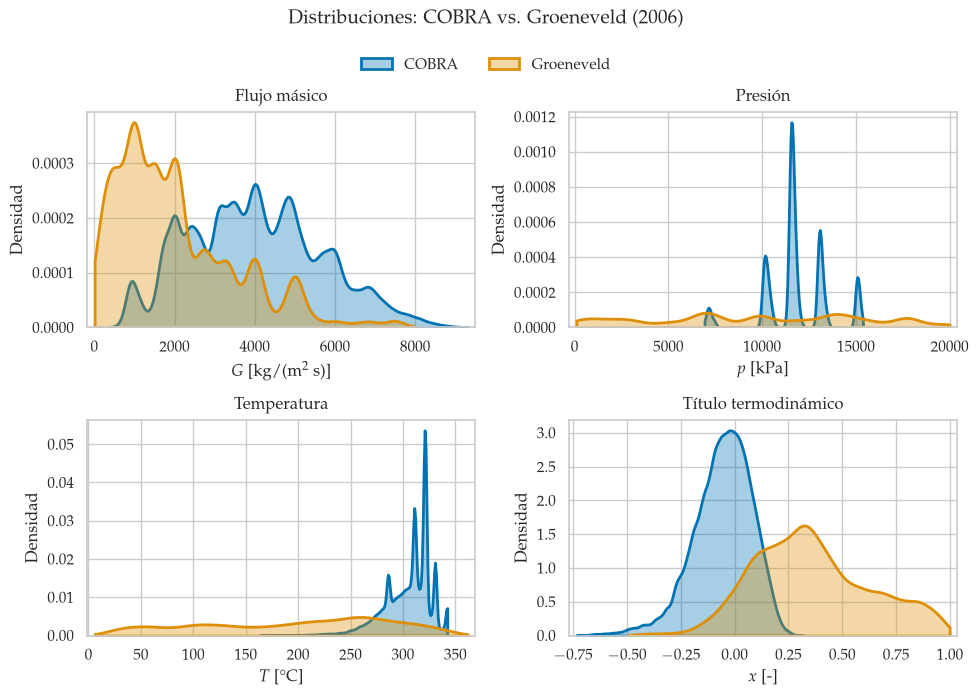
\includegraphics[width=\textwidth]{Figures/eda_cobra_groeneveld.png}
    \caption{Comparativa de distribuciones de datos de flujo másico, presión, temperatura y título termodinámico entre ensayos de un tubo de Groeneveld y todos los puntos de los ensayos numéricos con COBRA3-CP.}
    \label{fig:eda_cobra_groeneveld} 
\end{figure}

Entonces, se deben combinar los tensores de datos de entrenamiento de los datos de un tubo y de las simulaciones de COBRA3-CP para conformar el \texttt{Standard\allowbreak Scaler}. Las features adicionales que utiliza la red de alta fidelidad se escalan independientemente, por medio de un \texttt{Standard\allowbreak Scaler}. Para el valor del CHF también se pueden tener diferencias importantes, pero se realiza un escaleo independiente de las distribuciones, mediante la aplicación del logaritmo natural.

\subsection{Arquitectura del modelo}
Como se explicó previamente, el modelo planteado es una red de multifidelidad informada por física; se la denotará \texttt{MFPINN}. La \texttt{MFPINN} está compuesta por dos redes, una de baja fidelidad y otra de alta fidelidad. La de baja fidelidad es entrenada para predecir CHF en geometría de tubo, a partir de los datos crudos de las LUT de Groeneveld, y se la denotará \texttt{LFDNN}. Esta no tendrá información física, ya que se tiene una gran cantidad de datos, y un enfoque puro sobre ellos es suficiente. Su entrenamiento se realiza de forma previa, y sus pesos quedan congelados. Por otro lado, la componente de alta fidelidad sí utiliza información física, y se la denotará \texttt{HFPINN}. Los datos para su entrenamiento serán las simulaciones con COBRA3-CP de los ensayos experimentales de la Universidad de Columbia. En la figura \ref{fig:mfpinn} se presenta un esquema de la arquitectura de \texttt{MFPINN} explicada.

% Red neuronal multifidelidad:
%   - red de baja fidelidad (BF) pre-entrenada, con pesos fijos, que usa solo el
%     subconjunto de entradas x_1..x_n;
%   - red de alta fidelidad (AF) informada por la fisica (PINN), que usa todas las
%     entradas x_1..x_N mas la prediccion u_BF.
% La columna de entradas se dibuja UNA sola vez y es compartida: las entradas del
% subconjunto (recuadro sombreado) salen dos veces, hacia la red BF y hacia el bus
% de todas las entradas, mientras que las restantes salen solo hacia el bus.
%
% Fragmento para \input directo (sin el paquete standalone).
% NO necesita ninguna libreria de TikZ: solo \usepackage{tikz} y \usepackage{amsmath}.
% Uso tipico:
%   \begin{figure}[htbp]\centering
%     \resizebox{\textwidth}{!}{% Red neuronal multifidelidad:
%   - red de baja fidelidad (BF) pre-entrenada, con pesos fijos, que usa solo el
%     subconjunto de entradas x_1..x_n;
%   - red de alta fidelidad (AF) informada por la fisica (PINN), que usa todas las
%     entradas x_1..x_N mas la prediccion u_BF.
% La columna de entradas se dibuja UNA sola vez y es compartida: las entradas del
% subconjunto (recuadro sombreado) salen dos veces, hacia la red BF y hacia el bus
% de todas las entradas, mientras que las restantes salen solo hacia el bus.
%
% Fragmento para \input directo (sin el paquete standalone).
% NO necesita ninguna libreria de TikZ: solo \usepackage{tikz} y \usepackage{amsmath}.
% Uso tipico:
%   \begin{figure}[htbp]\centering
%     \resizebox{\textwidth}{!}{% Red neuronal multifidelidad:
%   - red de baja fidelidad (BF) pre-entrenada, con pesos fijos, que usa solo el
%     subconjunto de entradas x_1..x_n;
%   - red de alta fidelidad (AF) informada por la fisica (PINN), que usa todas las
%     entradas x_1..x_N mas la prediccion u_BF.
% La columna de entradas se dibuja UNA sola vez y es compartida: las entradas del
% subconjunto (recuadro sombreado) salen dos veces, hacia la red BF y hacia el bus
% de todas las entradas, mientras que las restantes salen solo hacia el bus.
%
% Fragmento para \input directo (sin el paquete standalone).
% NO necesita ninguna libreria de TikZ: solo \usepackage{tikz} y \usepackage{amsmath}.
% Uso tipico:
%   \begin{figure}[htbp]\centering
%     \resizebox{\textwidth}{!}{\input{Figures/mfnn_pinn.tex}}
%     \caption{...}\label{fig:mfnn_pinn}
%   \end{figure}
%
% Notas de implementacion (todas para que el fragmento no dependa del preambulo):
%  - Sin \usetikzlibrary aqui adentro: ejecutado en modo horizontal (dentro de un
%    \resizebox) deja ~55pt de espacios que ensanchan la caja del \input y hacen que
%    \resizebox empequenezca el dibujo; y no se puede encerrar en un grupo o \hbox
%    para absorberlos porque las definiciones de las librerias son locales.
%  - Sin la libreria backgrounds: los recuadros de las entradas se dibujan ANTES que
%    los circulos, de modo que el relleno queda debajo sin necesidad de capas.
%  - Sin la libreria fit: los recuadros de las redes se dan por coordenadas explicitas.
%  - Sin la libreria arrows.meta: las puntas son `stealth`, que ya trae pgf. Ademas se
%    escriben como -stealth y no con la clave >=, para no depender de que babel-spanish
%    tenga desactivado el shorthand `>`.
%  - Los tamanos de fuente son absolutos (\fontsize) para que la geometria no dependa
%    del tamano base del documento que hace el \input.
%  - El dibujo es casi cuadrado (15.3 x 15.3 cm) para que al escalarlo al ancho del
%    texto las etiquetas no queden diminutas.
\begin{figure}[hbtp]
  \centering
  \resizebox{\textwidth}{!}{
\begin{tikzpicture}[
  chico/.style={font=\fontsize{9}{11}\selectfont},
  % un unico estilo de circulo: entradas, neuronas y salidas miden todas lo mismo
  entrada/.style={circle,draw=black!70,fill=white,minimum size=0.9cm,inner sep=0pt,
                  font=\fontsize{9}{11}\selectfont},
  entradaG/.style={entrada},
  neurona/.style={entrada},
  salida/.style={entrada},
  syn/.style={draw=black!25,line width=0.3pt},
  reparto/.style={draw=black!45,line width=0.4pt},
  flujo/.style={-stealth,draw=black!75,line width=0.8pt},
  tronco/.style={draw=black!75,line width=0.8pt},
  bus/.style={-stealth,draw=black!75,line width=1.5pt},
  bloque/.style={rounded corners=2pt,draw=black!70,align=center,inner sep=5pt,
                 font=\fontsize{9}{11}\selectfont,text width=3.2cm},
  perdida/.style={bloque,fill=black!6},
  barra/.style={rounded corners=2pt,draw=black!70,fill=black!10,
                minimum width=0.6cm,minimum height=4.4cm,inner sep=0pt},
  grupoSub/.style={rounded corners=4pt,draw=black!40,fill=black!7},
  grupoResto/.style={rounded corners=4pt,draw=black!40,dash pattern=on 2pt off 1.5pt},
  grupoBF/.style={draw=black!45,dashed,rounded corners=6pt},
  grupoAF/.style={draw=black!70,rounded corners=6pt},
  etiqueta/.style={font=\fontsize{9}{11}\bfseries\selectfont,align=left,text width=5.2cm},
  nota/.style={font=\fontsize{8}{9.6}\selectfont,align=left},
  notac/.style={font=\fontsize{8}{9.6}\selectfont,align=center},
  bp/.style={-stealth,dashed,draw=black!60,line width=0.8pt},
]

%=============== COLUMNA DE ENTRADAS (UNICA Y COMPARTIDA) ==============
% los recuadros van primero para que el relleno quede por debajo de los circulos
\draw[grupoSub]   (-0.66, 0.09) rectangle (0.66, 4.06);
\draw[grupoResto] (-0.66,-3.21) rectangle (0.66,-0.39);

% subconjunto que ve la red de baja fidelidad
\node[entrada]  (e1)  at (0, 3.40) {$x_1$};
\node[entrada]  (e2)  at (0, 2.35) {$x_2$};
\node[chico]    (ev1) at (0, 1.55) {$\vdots$};
\node[entrada]  (en)  at (0, 0.75) {$x_n$};
% entradas restantes, exclusivas de la red de alta fidelidad
\node[entradaG] (er1) at (0,-1.05) {$x_{n+1}$};
\node[chico]    (ev2) at (0,-1.80) {$\vdots$};
\node[entrada]  (eN)  at (0,-2.55) {$x_N$};

% \node[notac,rotate=90] at (-1.35, 2.02) {primeras $n$\\ entradas};
% \node[notac,rotate=90] at (-1.35,-1.80) {entradas\\ restantes};

%=================== RED DE BAJA FIDELIDAD (BF) ========================
\foreach \j/\y in {1/3.07,2/2.02,3/0.97} {
  \node[neurona] (bf1-\j) at (2.6,\y) {};
  \node[neurona] (bf2-\j) at (4.1,\y) {};
}
\node[salida] (ubf) at (5.6,2.02) {$u_\text{LF}$};

% solo el subconjunto alimenta la red BF
\foreach \e in {e1,e2,en} {
  \foreach \j in {1,2,3} { \draw[syn] (\e) -- (bf1-\j); }
}
\foreach \i in {1,2,3} {
  \foreach \j in {1,2,3} { \draw[syn] (bf1-\i) -- (bf2-\j); }
  \draw[syn] (bf2-\i) -- (ubf);
}

\draw[grupoBF] (1.83,0.20) rectangle (6.37,3.84);
\node[etiqueta,anchor=south west] at (1.83,3.84)
  {Red de baja fidelidad $\theta_\text{LF}$ pre-entrenada};

%=========== BUS CON TODAS LAS ENTRADAS HACIA LA RED AF ================
% cada entrada, del subconjunto y de las restantes, se reparte al bus
\coordinate (nodoBus) at (2.6,-3.0);
\foreach \e in {e1,e2,en,er1,eN} { \draw[reparto] (\e) -- (nodoBus); }
\fill[black!75] (nodoBus) circle (1.6pt);

\draw[bus,rounded corners=3pt] (nodoBus) -- (5.9,-3.0) -- (5.9,-1.2) -- (7.30,-1.2);
\node[nota,anchor=north west] at (2.9,-3.4) {todas las entradas\\ $x_1,\dots,x_N$};

%=================== RED DE ALTA FIDELIDAD (AF) ========================
\node[barra] (concat) at (7.6,0) {};
\node[nota,rotate=90] at (7.6,0) {concatenación};

\foreach \j/\y in {1/1.70,2/0.57,3/-0.57,4/-1.70} {
  \node[neurona] (af1-\j) at (8.9,\y) {};
  \node[neurona] (af2-\j) at (10.4,\y) {};
}
\node[salida] (uaf) at (11.9,0) {$u_\text{HF}$};

\draw[flujo] (ubf.east) -- (7.30,1.3);
\foreach \j in {1,2,3,4} { \draw[syn] (concat.east) -- (af1-\j); }
\foreach \i in {1,2,3,4} {
  \foreach \j in {1,2,3,4} { \draw[syn] (af1-\i) -- (af2-\j); }
  \draw[syn] (af2-\i) -- (uaf);
}

\draw[grupoAF] (6.98,-2.52) rectangle (12.67,2.52);
\node[etiqueta,anchor=south west] at (6.98,2.52)
  {Red de alta fidelidad $\theta_\text{HF}$\\ informada por la física (PINN)};

%=============== RAMAS DE PÉRDIDA (FÍSICA Y DATOS) =====================
\node[bloque]  (ad)   at (4.6,-6.3)
  {Derivadas\\ automáticas\\ de $u_\text{HF}$ respecto\\ de las entradas};
\node[perdida] (lfis) at (4.6,-8.4)
  {$\mathcal{L}_{\text{fís}}=\big\|\mathcal{R}(u_\text{HF})\big\|^{2}$\\ residuo de la EDP};
\node[perdida,text width=3.4cm] (ldat) at (8.8,-6.3)
  {$\mathcal{L}_{\text{datos}}=\big\|u_\text{HF}-u^{*}\big\|^{2}$\\ $u^{*}$: datos medidos};
\node[perdida,text width=3.4cm] (ltot) at (8.8,-8.4)
  {$\mathcal{L}=\mathcal{L}_{\text{datos}}+\lambda\,\mathcal{L}_{\text{fís}}$};

% tronco desde u_AF, con derivacion hacia la rama de datos
\coordinate (bif) at (11.9,-4.9);
\draw[tronco] (uaf.south) -- (bif);
\draw[flujo,rounded corners=3pt] (bif) -- (4.6,-4.9) -- (ad.north);
\fill[black!75] (8.8,-4.9) circle (1.6pt);
\draw[flujo] (8.8,-4.9) -- (ldat.north);

\draw[flujo] (ad.south)   -- (lfis.north);
\draw[flujo] (ldat.south) -- (ltot.north);
\draw[flujo] (lfis.east)  -- (ltot.west);

%=================== RETROPROPAGACIÓN (SOLO RED AF) ====================
% vuelve por la derecha y entra al costado de la red AF, sin cruzar el tronco
\draw[bp,rounded corners=3pt]
  (ltot.east) -- (13.4,-8.4) -- (13.4,-1.8) -- (12.67,-1.8);
% \node[notac,anchor=north,text width=4.2cm] at (8.8,-9.3)
%   {retropropagación: sólo se\\ actualizan los pesos $\theta_{AF}$};

%============================ ACLARACIÓN ===============================
% \node[nota,anchor=north west,text width=4.0cm] at (-1.75,-4.9)
%   {la red BF sólo usa $x_1,\dots,x_n$; la red AF usa todas las entradas y
%    además $u_{BF}$};

\end{tikzpicture}
  }
  \caption{Esquema de la arquitectura de red neuronal de multifidelidad informada por física.}
  \label{fig:mfpinn}
\end{figure}
}
%     \caption{...}\label{fig:mfnn_pinn}
%   \end{figure}
%
% Notas de implementacion (todas para que el fragmento no dependa del preambulo):
%  - Sin \usetikzlibrary aqui adentro: ejecutado en modo horizontal (dentro de un
%    \resizebox) deja ~55pt de espacios que ensanchan la caja del \input y hacen que
%    \resizebox empequenezca el dibujo; y no se puede encerrar en un grupo o \hbox
%    para absorberlos porque las definiciones de las librerias son locales.
%  - Sin la libreria backgrounds: los recuadros de las entradas se dibujan ANTES que
%    los circulos, de modo que el relleno queda debajo sin necesidad de capas.
%  - Sin la libreria fit: los recuadros de las redes se dan por coordenadas explicitas.
%  - Sin la libreria arrows.meta: las puntas son `stealth`, que ya trae pgf. Ademas se
%    escriben como -stealth y no con la clave >=, para no depender de que babel-spanish
%    tenga desactivado el shorthand `>`.
%  - Los tamanos de fuente son absolutos (\fontsize) para que la geometria no dependa
%    del tamano base del documento que hace el \input.
%  - El dibujo es casi cuadrado (15.3 x 15.3 cm) para que al escalarlo al ancho del
%    texto las etiquetas no queden diminutas.
\begin{figure}[hbtp]
  \centering
  \resizebox{\textwidth}{!}{
\begin{tikzpicture}[
  chico/.style={font=\fontsize{9}{11}\selectfont},
  % un unico estilo de circulo: entradas, neuronas y salidas miden todas lo mismo
  entrada/.style={circle,draw=black!70,fill=white,minimum size=0.9cm,inner sep=0pt,
                  font=\fontsize{9}{11}\selectfont},
  entradaG/.style={entrada},
  neurona/.style={entrada},
  salida/.style={entrada},
  syn/.style={draw=black!25,line width=0.3pt},
  reparto/.style={draw=black!45,line width=0.4pt},
  flujo/.style={-stealth,draw=black!75,line width=0.8pt},
  tronco/.style={draw=black!75,line width=0.8pt},
  bus/.style={-stealth,draw=black!75,line width=1.5pt},
  bloque/.style={rounded corners=2pt,draw=black!70,align=center,inner sep=5pt,
                 font=\fontsize{9}{11}\selectfont,text width=3.2cm},
  perdida/.style={bloque,fill=black!6},
  barra/.style={rounded corners=2pt,draw=black!70,fill=black!10,
                minimum width=0.6cm,minimum height=4.4cm,inner sep=0pt},
  grupoSub/.style={rounded corners=4pt,draw=black!40,fill=black!7},
  grupoResto/.style={rounded corners=4pt,draw=black!40,dash pattern=on 2pt off 1.5pt},
  grupoBF/.style={draw=black!45,dashed,rounded corners=6pt},
  grupoAF/.style={draw=black!70,rounded corners=6pt},
  etiqueta/.style={font=\fontsize{9}{11}\bfseries\selectfont,align=left,text width=5.2cm},
  nota/.style={font=\fontsize{8}{9.6}\selectfont,align=left},
  notac/.style={font=\fontsize{8}{9.6}\selectfont,align=center},
  bp/.style={-stealth,dashed,draw=black!60,line width=0.8pt},
]

%=============== COLUMNA DE ENTRADAS (UNICA Y COMPARTIDA) ==============
% los recuadros van primero para que el relleno quede por debajo de los circulos
\draw[grupoSub]   (-0.66, 0.09) rectangle (0.66, 4.06);
\draw[grupoResto] (-0.66,-3.21) rectangle (0.66,-0.39);

% subconjunto que ve la red de baja fidelidad
\node[entrada]  (e1)  at (0, 3.40) {$x_1$};
\node[entrada]  (e2)  at (0, 2.35) {$x_2$};
\node[chico]    (ev1) at (0, 1.55) {$\vdots$};
\node[entrada]  (en)  at (0, 0.75) {$x_n$};
% entradas restantes, exclusivas de la red de alta fidelidad
\node[entradaG] (er1) at (0,-1.05) {$x_{n+1}$};
\node[chico]    (ev2) at (0,-1.80) {$\vdots$};
\node[entrada]  (eN)  at (0,-2.55) {$x_N$};

% \node[notac,rotate=90] at (-1.35, 2.02) {primeras $n$\\ entradas};
% \node[notac,rotate=90] at (-1.35,-1.80) {entradas\\ restantes};

%=================== RED DE BAJA FIDELIDAD (BF) ========================
\foreach \j/\y in {1/3.07,2/2.02,3/0.97} {
  \node[neurona] (bf1-\j) at (2.6,\y) {};
  \node[neurona] (bf2-\j) at (4.1,\y) {};
}
\node[salida] (ubf) at (5.6,2.02) {$u_\text{LF}$};

% solo el subconjunto alimenta la red BF
\foreach \e in {e1,e2,en} {
  \foreach \j in {1,2,3} { \draw[syn] (\e) -- (bf1-\j); }
}
\foreach \i in {1,2,3} {
  \foreach \j in {1,2,3} { \draw[syn] (bf1-\i) -- (bf2-\j); }
  \draw[syn] (bf2-\i) -- (ubf);
}

\draw[grupoBF] (1.83,0.20) rectangle (6.37,3.84);
\node[etiqueta,anchor=south west] at (1.83,3.84)
  {Red de baja fidelidad $\theta_\text{LF}$ pre-entrenada};

%=========== BUS CON TODAS LAS ENTRADAS HACIA LA RED AF ================
% cada entrada, del subconjunto y de las restantes, se reparte al bus
\coordinate (nodoBus) at (2.6,-3.0);
\foreach \e in {e1,e2,en,er1,eN} { \draw[reparto] (\e) -- (nodoBus); }
\fill[black!75] (nodoBus) circle (1.6pt);

\draw[bus,rounded corners=3pt] (nodoBus) -- (5.9,-3.0) -- (5.9,-1.2) -- (7.30,-1.2);
\node[nota,anchor=north west] at (2.9,-3.4) {todas las entradas\\ $x_1,\dots,x_N$};

%=================== RED DE ALTA FIDELIDAD (AF) ========================
\node[barra] (concat) at (7.6,0) {};
\node[nota,rotate=90] at (7.6,0) {concatenación};

\foreach \j/\y in {1/1.70,2/0.57,3/-0.57,4/-1.70} {
  \node[neurona] (af1-\j) at (8.9,\y) {};
  \node[neurona] (af2-\j) at (10.4,\y) {};
}
\node[salida] (uaf) at (11.9,0) {$u_\text{HF}$};

\draw[flujo] (ubf.east) -- (7.30,1.3);
\foreach \j in {1,2,3,4} { \draw[syn] (concat.east) -- (af1-\j); }
\foreach \i in {1,2,3,4} {
  \foreach \j in {1,2,3,4} { \draw[syn] (af1-\i) -- (af2-\j); }
  \draw[syn] (af2-\i) -- (uaf);
}

\draw[grupoAF] (6.98,-2.52) rectangle (12.67,2.52);
\node[etiqueta,anchor=south west] at (6.98,2.52)
  {Red de alta fidelidad $\theta_\text{HF}$\\ informada por la física (PINN)};

%=============== RAMAS DE PÉRDIDA (FÍSICA Y DATOS) =====================
\node[bloque]  (ad)   at (4.6,-6.3)
  {Derivadas\\ automáticas\\ de $u_\text{HF}$ respecto\\ de las entradas};
\node[perdida] (lfis) at (4.6,-8.4)
  {$\mathcal{L}_{\text{fís}}=\big\|\mathcal{R}(u_\text{HF})\big\|^{2}$\\ residuo de la EDP};
\node[perdida,text width=3.4cm] (ldat) at (8.8,-6.3)
  {$\mathcal{L}_{\text{datos}}=\big\|u_\text{HF}-u^{*}\big\|^{2}$\\ $u^{*}$: datos medidos};
\node[perdida,text width=3.4cm] (ltot) at (8.8,-8.4)
  {$\mathcal{L}=\mathcal{L}_{\text{datos}}+\lambda\,\mathcal{L}_{\text{fís}}$};

% tronco desde u_AF, con derivacion hacia la rama de datos
\coordinate (bif) at (11.9,-4.9);
\draw[tronco] (uaf.south) -- (bif);
\draw[flujo,rounded corners=3pt] (bif) -- (4.6,-4.9) -- (ad.north);
\fill[black!75] (8.8,-4.9) circle (1.6pt);
\draw[flujo] (8.8,-4.9) -- (ldat.north);

\draw[flujo] (ad.south)   -- (lfis.north);
\draw[flujo] (ldat.south) -- (ltot.north);
\draw[flujo] (lfis.east)  -- (ltot.west);

%=================== RETROPROPAGACIÓN (SOLO RED AF) ====================
% vuelve por la derecha y entra al costado de la red AF, sin cruzar el tronco
\draw[bp,rounded corners=3pt]
  (ltot.east) -- (13.4,-8.4) -- (13.4,-1.8) -- (12.67,-1.8);
% \node[notac,anchor=north,text width=4.2cm] at (8.8,-9.3)
%   {retropropagación: sólo se\\ actualizan los pesos $\theta_{AF}$};

%============================ ACLARACIÓN ===============================
% \node[nota,anchor=north west,text width=4.0cm] at (-1.75,-4.9)
%   {la red BF sólo usa $x_1,\dots,x_n$; la red AF usa todas las entradas y
%    además $u_{BF}$};

\end{tikzpicture}
  }
  \caption{Esquema de la arquitectura de red neuronal de multifidelidad informada por física.}
  \label{fig:mfpinn}
\end{figure}
}
%     \caption{...}\label{fig:mfnn_pinn}
%   \end{figure}
%
% Notas de implementacion (todas para que el fragmento no dependa del preambulo):
%  - Sin \usetikzlibrary aqui adentro: ejecutado en modo horizontal (dentro de un
%    \resizebox) deja ~55pt de espacios que ensanchan la caja del \input y hacen que
%    \resizebox empequenezca el dibujo; y no se puede encerrar en un grupo o \hbox
%    para absorberlos porque las definiciones de las librerias son locales.
%  - Sin la libreria backgrounds: los recuadros de las entradas se dibujan ANTES que
%    los circulos, de modo que el relleno queda debajo sin necesidad de capas.
%  - Sin la libreria fit: los recuadros de las redes se dan por coordenadas explicitas.
%  - Sin la libreria arrows.meta: las puntas son `stealth`, que ya trae pgf. Ademas se
%    escriben como -stealth y no con la clave >=, para no depender de que babel-spanish
%    tenga desactivado el shorthand `>`.
%  - Los tamanos de fuente son absolutos (\fontsize) para que la geometria no dependa
%    del tamano base del documento que hace el \input.
%  - El dibujo es casi cuadrado (15.3 x 15.3 cm) para que al escalarlo al ancho del
%    texto las etiquetas no queden diminutas.
\begin{figure}[hbtp]
  \centering
  \resizebox{\textwidth}{!}{
\begin{tikzpicture}[
  chico/.style={font=\fontsize{9}{11}\selectfont},
  % un unico estilo de circulo: entradas, neuronas y salidas miden todas lo mismo
  entrada/.style={circle,draw=black!70,fill=white,minimum size=0.9cm,inner sep=0pt,
                  font=\fontsize{9}{11}\selectfont},
  entradaG/.style={entrada},
  neurona/.style={entrada},
  salida/.style={entrada},
  syn/.style={draw=black!25,line width=0.3pt},
  reparto/.style={draw=black!45,line width=0.4pt},
  flujo/.style={-stealth,draw=black!75,line width=0.8pt},
  tronco/.style={draw=black!75,line width=0.8pt},
  bus/.style={-stealth,draw=black!75,line width=1.5pt},
  bloque/.style={rounded corners=2pt,draw=black!70,align=center,inner sep=5pt,
                 font=\fontsize{9}{11}\selectfont,text width=3.2cm},
  perdida/.style={bloque,fill=black!6},
  barra/.style={rounded corners=2pt,draw=black!70,fill=black!10,
                minimum width=0.6cm,minimum height=4.4cm,inner sep=0pt},
  grupoSub/.style={rounded corners=4pt,draw=black!40,fill=black!7},
  grupoResto/.style={rounded corners=4pt,draw=black!40,dash pattern=on 2pt off 1.5pt},
  grupoBF/.style={draw=black!45,dashed,rounded corners=6pt},
  grupoAF/.style={draw=black!70,rounded corners=6pt},
  etiqueta/.style={font=\fontsize{9}{11}\bfseries\selectfont,align=left,text width=5.2cm},
  nota/.style={font=\fontsize{8}{9.6}\selectfont,align=left},
  notac/.style={font=\fontsize{8}{9.6}\selectfont,align=center},
  bp/.style={-stealth,dashed,draw=black!60,line width=0.8pt},
]

%=============== COLUMNA DE ENTRADAS (UNICA Y COMPARTIDA) ==============
% los recuadros van primero para que el relleno quede por debajo de los circulos
\draw[grupoSub]   (-0.66, 0.09) rectangle (0.66, 4.06);
\draw[grupoResto] (-0.66,-3.21) rectangle (0.66,-0.39);

% subconjunto que ve la red de baja fidelidad
\node[entrada]  (e1)  at (0, 3.40) {$x_1$};
\node[entrada]  (e2)  at (0, 2.35) {$x_2$};
\node[chico]    (ev1) at (0, 1.55) {$\vdots$};
\node[entrada]  (en)  at (0, 0.75) {$x_n$};
% entradas restantes, exclusivas de la red de alta fidelidad
\node[entradaG] (er1) at (0,-1.05) {$x_{n+1}$};
\node[chico]    (ev2) at (0,-1.80) {$\vdots$};
\node[entrada]  (eN)  at (0,-2.55) {$x_N$};

% \node[notac,rotate=90] at (-1.35, 2.02) {primeras $n$\\ entradas};
% \node[notac,rotate=90] at (-1.35,-1.80) {entradas\\ restantes};

%=================== RED DE BAJA FIDELIDAD (BF) ========================
\foreach \j/\y in {1/3.07,2/2.02,3/0.97} {
  \node[neurona] (bf1-\j) at (2.6,\y) {};
  \node[neurona] (bf2-\j) at (4.1,\y) {};
}
\node[salida] (ubf) at (5.6,2.02) {$u_\text{LF}$};

% solo el subconjunto alimenta la red BF
\foreach \e in {e1,e2,en} {
  \foreach \j in {1,2,3} { \draw[syn] (\e) -- (bf1-\j); }
}
\foreach \i in {1,2,3} {
  \foreach \j in {1,2,3} { \draw[syn] (bf1-\i) -- (bf2-\j); }
  \draw[syn] (bf2-\i) -- (ubf);
}

\draw[grupoBF] (1.83,0.20) rectangle (6.37,3.84);
\node[etiqueta,anchor=south west] at (1.83,3.84)
  {Red de baja fidelidad $\theta_\text{LF}$ pre-entrenada};

%=========== BUS CON TODAS LAS ENTRADAS HACIA LA RED AF ================
% cada entrada, del subconjunto y de las restantes, se reparte al bus
\coordinate (nodoBus) at (2.6,-3.0);
\foreach \e in {e1,e2,en,er1,eN} { \draw[reparto] (\e) -- (nodoBus); }
\fill[black!75] (nodoBus) circle (1.6pt);

\draw[bus,rounded corners=3pt] (nodoBus) -- (5.9,-3.0) -- (5.9,-1.2) -- (7.30,-1.2);
\node[nota,anchor=north west] at (2.9,-3.4) {todas las entradas\\ $x_1,\dots,x_N$};

%=================== RED DE ALTA FIDELIDAD (AF) ========================
\node[barra] (concat) at (7.6,0) {};
\node[nota,rotate=90] at (7.6,0) {concatenación};

\foreach \j/\y in {1/1.70,2/0.57,3/-0.57,4/-1.70} {
  \node[neurona] (af1-\j) at (8.9,\y) {};
  \node[neurona] (af2-\j) at (10.4,\y) {};
}
\node[salida] (uaf) at (11.9,0) {$u_\text{HF}$};

\draw[flujo] (ubf.east) -- (7.30,1.3);
\foreach \j in {1,2,3,4} { \draw[syn] (concat.east) -- (af1-\j); }
\foreach \i in {1,2,3,4} {
  \foreach \j in {1,2,3,4} { \draw[syn] (af1-\i) -- (af2-\j); }
  \draw[syn] (af2-\i) -- (uaf);
}

\draw[grupoAF] (6.98,-2.52) rectangle (12.67,2.52);
\node[etiqueta,anchor=south west] at (6.98,2.52)
  {Red de alta fidelidad $\theta_\text{HF}$\\ informada por la física (PINN)};

%=============== RAMAS DE PÉRDIDA (FÍSICA Y DATOS) =====================
\node[bloque]  (ad)   at (4.6,-6.3)
  {Derivadas\\ automáticas\\ de $u_\text{HF}$ respecto\\ de las entradas};
\node[perdida] (lfis) at (4.6,-8.4)
  {$\mathcal{L}_{\text{fís}}=\big\|\mathcal{R}(u_\text{HF})\big\|^{2}$\\ residuo de la EDP};
\node[perdida,text width=3.4cm] (ldat) at (8.8,-6.3)
  {$\mathcal{L}_{\text{datos}}=\big\|u_\text{HF}-u^{*}\big\|^{2}$\\ $u^{*}$: datos medidos};
\node[perdida,text width=3.4cm] (ltot) at (8.8,-8.4)
  {$\mathcal{L}=\mathcal{L}_{\text{datos}}+\lambda\,\mathcal{L}_{\text{fís}}$};

% tronco desde u_AF, con derivacion hacia la rama de datos
\coordinate (bif) at (11.9,-4.9);
\draw[tronco] (uaf.south) -- (bif);
\draw[flujo,rounded corners=3pt] (bif) -- (4.6,-4.9) -- (ad.north);
\fill[black!75] (8.8,-4.9) circle (1.6pt);
\draw[flujo] (8.8,-4.9) -- (ldat.north);

\draw[flujo] (ad.south)   -- (lfis.north);
\draw[flujo] (ldat.south) -- (ltot.north);
\draw[flujo] (lfis.east)  -- (ltot.west);

%=================== RETROPROPAGACIÓN (SOLO RED AF) ====================
% vuelve por la derecha y entra al costado de la red AF, sin cruzar el tronco
\draw[bp,rounded corners=3pt]
  (ltot.east) -- (13.4,-8.4) -- (13.4,-1.8) -- (12.67,-1.8);
% \node[notac,anchor=north,text width=4.2cm] at (8.8,-9.3)
%   {retropropagación: sólo se\\ actualizan los pesos $\theta_{AF}$};

%============================ ACLARACIÓN ===============================
% \node[nota,anchor=north west,text width=4.0cm] at (-1.75,-4.9)
%   {la red BF sólo usa $x_1,\dots,x_n$; la red AF usa todas las entradas y
%    además $u_{BF}$};

\end{tikzpicture}
  }
  \caption{Esquema de la arquitectura de red neuronal de multifidelidad informada por física.}
  \label{fig:mfpinn}
\end{figure}


La \texttt{HFPINN} entrena con los datos de las simulaciones con COBRA3-CP; cada una de ellas provee datos en 151 nodos axiales y 60 subcanales, para un total de 9060 datos por ensayo. Por otro lado, la información provista por los ensayos de Columbia provee 1 dato por ensayo, correspondiente al punto, desconocido, en el que comienza el DNB. Se tiene entonces un desajuste de dimensionalidad entre el producto de la red al evaluar en los ensayos numéricos y lo medido en los ensayos reales:
\begin{equation}
    \underbrace{\mathbf{y} \in \mathbb{R}^{9060}}_{\text{campo predicho}}
    \quad\longrightarrow\quad
    \underbrace{\hat{y} \in \mathbb{R}}_{\text{campo medido}}.
    \label{eq:dim_red}
\end{equation}
La flecha en la ecuación \ref{eq:dim_red} es la reducción de dimensionalidad que se debe hacer antes de poder comparar contra los datos experimentales. La elección natural es el mínimo, ya que el DNB ocurre en el nodo más limitante del bundle. Pero, en cuanto a la optimización numérica, la utilización del mínimo es poco eficiente, e incluso puede hacer imposible el entrenamiento de un modelo de red neuronal, ya que el mínimo genera un gradiente \textit{one-hot}:
\begin{equation}
    \frac{\partial}{\partial y_j}\min_i y_i =
    \begin{cases}
    1 & \text{si } j = \arg\min_i y_i \\
    0 & \text{en caso contrario}
    \end{cases}.
\end{equation}
De esta forma el optimizador sólo recibe información del punto mínimo. Adicionalmente, al comenzar el entrenamiento, el punto que resulta mínimo es completamente aleatorio, por lo que es muy fácil condicionar negativamente la red y que esta no pueda salir del mínimo inicial.

Se plantea entonces utilizar un enfoque de mínimo suave o \textit{softmin}, que permita utilizar una mayor cantidad de nodos para el aprendizaje. Un problema similar que utiliza este enfoque es el promedio ponderado o \textit{attention pooling} propuesto por Ilse \citep{ilse2018attention} en el contexto de MIL (del inglés, \textit{Multiple Instance Learning}). Se propone utilizar un softmin de la forma:
\begin{equation}
    \mathrm{softmin}_\tau (\mathbf{y}) = \sum_i w_i y_i,
\end{equation}
donde $w_i$ son los pesos para ponderar las distintas predicciones. En el trabajo de Ilse los pesos se aprenden con una red de atención aparte, pero en este trabajo se utiliza el propio campo predicho, a través de la función softmax de Bridle \citep{bridle1990softmax} y el parámetro de temperatura propuesto por Hinton, Vinyals y Dean \citep{hinton2015distilling}:
\begin{equation}
    w_i = \mathrm{softmax}\left(-\frac{\mathbf{y}}{\tau}\right)_i .
\end{equation}
De esta forma, los nodos con baja predicción se ponderan con un mayor peso que los nodos con predicciones altas. El sesgo de esta concentración es controlado por el parámetro de temperatura $\tau$, que viene dado a partir del desvío estándar del vector de predicción:
\begin{equation}
    \tau = \alpha \cdot \mathrm{std}(\mathbf{y}).
\end{equation}
El parámetro $\alpha$ permite controlar la temperatura con la evolución del entrenamiento, y se lo controla por medio de un recocido o \textit{annealing}, que lo recorre geométricamente desde $\alpha_0$ hasta $\alpha_f$.

Para evaluar si la temperatura $\tau$ a la que converge el entrenamiento es o no correcta, se debe analizar sobre cuántos nodos se está promediando realmente. Para ello, se computa el número efectivo de nodos, que viene dado por la exponencial de la entropía de los pesos:
\begin{equation}
    N_\mathrm{eff} = \exp\left[ -\sum_i w_i\,\log(w_i) \right].
\end{equation}
Esta definición es el número de Hill de orden 1 \citep{hill1973diversity}, la forma estándar de obtener un conteo efectivo a partir de una entropía. Si el entrenamiento es satisfactorio, $N_\mathrm{eff}$ debe ser menor a 5 para su final.

Esta metodología, además de solucionar el problema del gradiente one-hot, tiene la ventaja de, al ser una combinación convexa de los $y_i$, estar acotada superiormente por la media de la predicción. Esto asegura que el valor predicho sea un valor físicamente válido y sin sesgo dependiente de la cantidad de nodos utilizados.

En cuanto a la información física que se le brindará a la \texttt{HFPINN}, se debe notar que no es posible hacer un planteo tradicional de PINN que provea una ecuación diferencial de conservación de alguna cantidad como función de pérdida. Esto es así puesto que la variable a predecir, el CHF, no responde a una ecuación de conservación, sino que es una propiedad del estado termodinámico y la geometría. Se podría realizar el ejercicio de proveer a la red de, por ejemplo, la ecuación de conservación de la energía. Esto haría que la red aprenda que siempre que le den un set de datos locales, los mismos corresponden a una condición de CHF, ya que la red fue entrenada con casos en que se tiene DNB. Pero en el campo de aplicación del modelo, se busca estimar el CHF sin estar en DNB.

Se plantean entonces, distintos tipos de ecuaciones diferenciales a satisfacer por el modelo. Se tendrán relaciones monotónicas, de derivada cruzada, de convexidad y de coincidencia entre la predicción del modelo y la simulación de COBRA3-CP.

Las relaciones monotónicas del CHF con las variables de entrada implementadas son: positiva con el flujo másico, negativa con el título termodinámico y negativa con la presión. Estas relaciones tienen fundamento físico y aseguran que las salidas de la red en condiciones de extrapolación mantengan sentido físico. Vale aclarar que esta última es válida para el rango de aplicación de reactores PWR o PHWR, es decir, por encima de 100 bar.

Se implementa una relación negativa con la derivada cruzada respecto del flujo másico y el título termodinámico, fundamentada en que a mayor flujo másico, la caída del CHF con el título termodinámico es más pronunciada. Esto es consistente con las estimaciones de las LUT de Groeneveld.

En cuanto a la relación de convexidad, se plantea una derivada segunda positiva del CHF respecto del título termodinámico para la zona de alto título ($x>0,2$). Si bien de la figura \ref{fig:eda_cobra_groeneveld} puede afirmarse que se tienen pocos datos que se encuentran en esa región, esta restricción es útil en puntos de colocación para asegurar que el modelo no obtiene resultados indeseados al extrapolar fuera de los datos de entrenamiento.

Por último, se realiza la comparación de la derivada axial del valor predicho de CHF calculada por dos métodos. En primer lugar se computa la derivada observada como:
\begin{equation}
    \left. \frac{d\mathrm{CHF}}{dz} \right|_\text{obs} = \frac{\mathrm{CHF}_{z_{i+1}} - \mathrm{CHF}_{z_{i}}}{z_{i+1} - z_i}.
\end{equation}
Luego la derivada por regla de la cadena viene dada por:
\begin{equation}
    \left. \frac{d\mathrm{CHF}}{dz} \right|_\text{cadena} = \sum_{j\in\mathrm{feats}} \frac{\partial \mathrm{CHF}}{\partial j} \frac{dj}{dz} ,
\end{equation}
donde las derivadas de las variables respecto de la coordenada axial $\nicefrac{dj}{dz}$ fueron computadas previamente a partir de los resultados de las simulaciones con COBRA3-CP. De esta manera se penaliza que la red invente dependencias axiales que no provengan de las condiciones locales, y de alguna forma, es una expresión de la hipótesis de condiciones locales como PDE.

Para el entrenamiento del modelo, en primer lugar se entrena la \texttt{LFDNN} con sus datos. Su entrenamiento es estándar y puede realizarse con optimizador Adam y métrica MSE.
Luego, con los pesos de la \texttt{LFDNN} congelados, se entrena la \texttt{HFPINN} con la estructura completa de la \texttt{MFPINN}. Para ello se realizaron pruebas para determinar si es necesario, debido a las restricciones tipo PINN, un optimizador de segundo orden como L-BFGS \citep{liu1989lbfgs}. El resultado de las mismas se expone en el capítulo \ref{Chapter4}.

\subsection{Evaluación del modelo}
Para la evaluación del modelo se utilizaron las métricas estadísticas tradicionales en conjunto con métricas particulares al problema en particular. Las métricas estadísticas utilizadas son el error cuadrático medio (MSE, del inglés \textit{Mean Squared Error}), su raíz (RMSE, del inglés \textit{Root Mean Squared Error}), y el coeficiente de correlación $\mathrm{R}^2$. En cuanto a la métricas particulares al problema, se utiliza el $\mathrm{DNBR}_\mathrm{min}$ del diseño termohidráulico de la \cna{}, explicado en detalle en \citep{IFS_CNA2, invap_thdesign}. Este es el valor para el cual, si la predicción de DNBR está por encima, se asegura con 95\% de probabilidad y confianza que no se tiene DNB. Se define como:
\begin{equation}
    \mathrm{DNBR}_\mathrm{min} = \overline{\mathrm{DNBR}} + k_{95}\cdot \sigma(\mathrm{DNBR}) ,
\end{equation}
donde DNBR son las predicciones en las condiciones de los ensayos de la Universidad de Columbia, y $k_{95}$ es el intervalo de tolerancia de una distribución normal para asegurar 95\% de probabilidad y confianza según la cantidad de observaciones \citep{nist_e_handbook_tolerance}. Se compara con la metodología actual (LUT + TMF), que obtiene $\mathrm{DNBR}_\mathrm{min} = 1,21$.